%%%%%%%%%%%%%%%%%%%%%%%%%%%%%%%%%%%%%%%%%%%%%%%%%%%%%%%%%%%%%%%%%%%%%%%%%%%%%%%
% Descripción: Template para la generación de la tesis de la MDIAE
% Autor: 
% Fecha: 20/05/2016
%%%%%%%%%%%%%%%%%%%%%%%%%%%%%%%%%%%%%%%%%%%%%%%%%%%%%%%%%%%%%%%%%%%%%%%%%%%%%%%

%%%%%%%%%%%%%%%%%%%%%%%%%%%%%%%%%%%%%%%%%%%%%%%%%%%%%%%%%%%%%%%%%%%%%%%%%%%%%%%
%%	PARA INSERTAR FIGURAS USAR LA FUNCION PREDEFINIDA \imagen
%%
%%      \imagen{escala}{path imagen}{caption}{referencia}
%%
%% donde:
%% 	* escala: es un valor numérico. Preferentemente usar valores entre 0 y 1.
%%		(ejemplo: 0.2)
%% 	* path: imagen es el directorio relativo donde se encuentra la imagen
%%		(ejemplo: Figures/Logos/conae-logo.png)
%%	* caption: texto de pie de figura.
%%	* referencia: texto que sirve para citar la figura. 
%%		(ejemplo: fig:conaelogo) luego se podrá hacer referencia \ref{fig:conaelogo}
%%%%%%%%%%%%%%%%%%%%%%%%%%%%%%%%%%%%%%%%%%%%%%%%%%%%%%%%%%%%%%%%%%%%%%%%%%%%%%%

%------------------------------------------------------------------------------
% Formato del documento
\documentclass[11pt, a4paper, twoside]{report}

%------------------------------------------------------------------------------
% TEMPLATE MDIAE (ACÁ SE ENCUETRAN LAS CUSTOMIZACIONES)
% Remitirse al archivo mdiaedoc.sty
\usepackage{mdiaedoc}

%Configuración de los márgenes
\usepackage[top=3cm, bottom=3cm, left=2.5cm, right=1.5cm]{geometry}

\usepackage{color}
%------------------------------------------------------------------------------
% Esto no se usa (YA ESTA DEFINIDO EN EL TEMPLATE)
%\usepackage{setspace}

%%%%%%%%%%%%%%%%%%%%%%%%%%%%%%%%%%%%%%%%%%%%%%%%%%%%%%%%%%%%%%%%%%%%%%%%%%%%%%%
% COMIENZO DEL DOCUMENTO
%%%%%%%%%%%%%%%%%%%%%%%%%%%%%%%%%%%%%%%%%%%%%%%%%%%%%%%%%%%%%%%%%%%%%%%%%%%%%%%
\begin{document}

\makeatletter
\author{Elbio Enrique Zapata}
\makeatother

%------------------------------------------------------------------------------
% PORTADA
\portadatesis{Detección de Patrones en imágenes satelitales utilizando Metodologías de Visión Artificial}{Elbio E. Zapata}{UNIVERSIDAD NACIONAL DE LA MATANZA}{TBD, 
2018}{2017}{Dr.Jorge Sánchez}{FaMAF, Cordoba, Argentina}


\pagenumbering{gobble}

%\chapter*{Abstract}
\label{chap:abstract}





















\textbf{Keywords:Computer Vision, Pattern Recognition}
%\chapter*{Resumen}
\label{chap:resumen}

El campo del aprendizaje automático en el reconocimiento de patrones es un área de estudio que en la actualidad es de gran interés para la comunidad científica como así también para la sociedad; hoy en día vemos como los avances de las tecnologías impacta en una gran proporción al mundo en el que vivimos desde aplicaciones de ocio en el celular hasta herramientas que proporcionan mejora en los procesos automatizando de manera eficiente los datos.

En la industria satelital existe gran cantidad de información que aún no fueron explotadas, en épocas pasadas esto se debía a los grandes costos que tienen el desarrollo de un satélite como también el acceso y procesado de los datos. En la actualidad no es así, esto se debió gracias a los desarrollos de pequeños satélites \textit{CubeSat} que permitieron abaratar costos y por otra parte el avance del poder de computo.

Tomando como ejemplo lo expuesto anteriormente el objetivo de esta tesis es realizar una evaluación experimental haciendo uso  de herramientas de Visión Artificial y Aprendizaje Automático en la detección de patrones sobre imágenes satelitales. 
Por otra parte, debido a la gran varianza de las imágenes y la gran cantidad de información que puede entregar una imagen satelital con diferentes bandas se realizo una manipulación exhaustiva de los datos con el fin de optimizar las predicciones de los algoritmos entrenados. 

La información extraída de una imagen satelital puede ser de gran ayuda para optimizar el almacenamiento de un CubeSat, servir de apoyo en el mecanismo de apuntamiento del satélite dando también un punto de partida para la realización de nuevas aplicaciones usando estos nuevos enfoques sobre imágenes satelitales.

Para concluir se realizaron diversos entrenamientos y cálculos de métricas para obtener una evaluación cualitativa de los modelos creados con el fin de obtener una conclusión del baseline propuesto en esta tesis. Los resultados obtenidos nos hace ver que los nuevos enfoques desarrollados en el área pueden sacar provecho en el ambiente satelital haciendo mas efectivo y automático los procesos de extracción de características de interés de una imagen satelital.

%%%% Texto (no menos de 200 palabras)

\textbf{Palabras clave: CubeSat, Visión Artificial, Detección de Patrones, Aprendizaje Automático, teledeteccion}


%\chapter*{Agradecimientos}
\label{chap:agradecimientos}
 %% OPCIONAL

\tabladecontenidos

\chapter*{Lista de acrónimos}
\label{chap:acronimos}

\begin{acronym}
% siglas de instituciones
\acro{cett}[CETT]{Centro Espacial Teófilo Tabanera}
\acro{conae}[CONAE]{Comisión Nacional de Actividades Espaciales}
\acro{fs}[FS2017]{Formador Satelital 2017}
\acro{sur}[SUR]{SUR Emprendimientos Tecnológicos}
\acro{unlam}[UNLaM]{Universidad Nacional de la Matanza}
% siglas Machine Learning
\acro{cv}[CV]{Computer Vision}
\acro{ml}[ML]{Machine Learning}
\acro{dl}[DL]{Deep Learning}
\acro{cnn}[CNN]{Redes neuronales convolucionales}
\acro{rp}[RP]{Regions Proposal}
\acro{nms}[NMS]{Non-Maxima Suppression}
% herramientas y demases
\acro{svm}[SVM]{Máquinas de vectores de soporte}
\acro{opencv}[OpenCV]{Open Source Computer Vision Library}
\acro{modis}[MODIS]{Espectrorradiómetro de imágenes de media resolución}
\acro{viirs}[VIIRS]{Radiómetro infrarrojo visible}
\acro{uav}[UAVs]{Vehículo aéreo no tripulado}
\acro{gps}[GPS]{Sistema de Posicionamiento Global}
\acro{nasa}[NASA]{National Aeronautics and Space Administration}
\acro{spheres}[SPHERES]{Synchronize Position Hold Engage and Reorient Experimental Satellite}
\acro{asitrov} [ASIROV]{Docking and Capture of Satellites through computer vision}
\end{acronym}



%------------------------------------------------------------------------------
% Numeración arábiga a partir de este punto
\pagenumbering{arabic}
\setcounter{page}{1}

%\chapter{Introducción}\label{chap:introduccion}

Este capítulo abordara los principales conceptos relacionados al trabajo realizado de esta tesis, comenzando con una descripción del marco de trabajo de investigación, el objetivo principal, los objetivos secundarios, fundamentos y motivación que nos llevo a realizar la pregunta de investigación, se dará un resumen del estado del arte de la temática en el ámbito espacial describiendo la metodología empleada para el desarrollo de software implementado.  Para finalizar se describe los capítulos posteriores que dan al lector una guía de como esta organizada la tesis.


\section{Contexto de la tesis}\label{sec:contexto}
El presente trabajo se realizó para recibir el grado de \textbf{\textit{Maestría en desarrollos informáticos de aplicación espacial}}. El mismo se encuadra dentro del Plan Nacional Espacial Argentino vigente (2004-2015), a través de \ac{conae} en conjunto con la unidad académica \ac{unlam} y la unidad de desarrollo \ac{sur}.

Esta investigación se centra en aplicar  algoritmos de \textit{Visión por computadora} (\ac{cv} por sus siglas en ingles)  y \textit{Aprendizaje automático} (\ac{ml} por sus siglas en ingles) para la localización y reconocimiento de objetos en una imagen satelital.


\section{Objetivo principal de la tesis}\label{sec:obj_general}

El objetivo principal de este trabajo de tesis es, analizar y utilizar algoritmos para el  reconocimiento de patrones en imágenes satelitales de la superficie terrestre haciendo uso de metodologías de \ac{cv} y \ac{ml} buscando realizar una prototipo experimental de estas técnicas computacionales.


\subsection{Objetivos específicos }\label{sub:obj_especifico}
A continuación se expondrá los objetivos específicos que permiten en su conjunto establecer los pasos a seguir para  cumplir con el objetivo primario:
\begin{itemize}
 \item Investigar técnicas de \ac{cv} y \ac{ml} aplicadas al reconocimiento de patrones.
 \item Evaluar la factibilidad de ser implementadas sobre imágenes satelitales.
 \item Desarrollar un prototipo de software que permita detectar patrones utilizando diferentes técnicas computacionales de \ac{cv} y \ac{ml}.
 \item Validación de los resultados obtenidos.
\end{itemize}


\section{Fundamentación/motivación}\label{sec:fundamentacion}

Partiendo del objetivo principal, la presente investigación como se desarrollo anteriormente se centra en evaluar diversas técnicas de \ac{cv} y \ac{ml} aplicadas a imágenes satelitales terrestres. Las regiones de interés de estudio que se aborda en esta tesis son:
\begin{itemize}
	\item Golfo San Matías (Rio Negro-Argentina).
	\item Laguna Mar Chiquita (Córdoba-Argentina).
\end{itemize}

Las imágenes que se utilizaron para el desarrollo fueron obtenidas de los instrumento  \ac{viirs}. Estas imágenes se asemejan a las características de la cámara NIR/SWIR del SABIA-MAR(Satélite Argentino Brasileño para Información del Mar) cuya factibilidad de ser usada en un CubeSat fue evaluada en el marco del proyecto integrador \ac{fs} de \ac{conae}.

El reconocimiento de patrones en imágenes es un área que en la actualidad se incremento con la aparición de nuevas técnicas y de los avances de poder de cómputo. La aplicación de técnicas computacionales tanto de  \ac{cv} y \ac{ml} en reconocimiento de patrones  en tierra y en vuelo, nos permite aprovechar la información contenida en la imagen  automatizando el proceso de extracción de los datos.

Diversas son las ventajas que nos permitirán realizar estos nuevos enfoques computacionales en el área espacial. Los principales beneficios al aplicar técnicas de \ac{cv} y \ac{ml} son: 
\begin{itemize}
\item \textbf{Calibración y apuntamiento}: brindar un mecanismo de apoyo para colaborar con el apuntamiento y la calibración óptica del satélite; mayormente para CubeSat, satélites de menor tamaño, que no poseen un mecanismo eficiente de determinación orbital como un Star-tracker o GPS debido a que son satélites de bajo costo además con relación al tamaño del mismo; con esto se podrá mejorar el apuntamiento detectando las regiones y comparando con los planes de pasadas  establecidos, a la vez dar soporte para poder calibrar la cámara óptica de acuerdo a la región.
\item \textbf{Almacenamiento en memoria}: una de las grandes desventajas que tienen los satélites, es la escasez de recursos en vuelo, teniendo un mecanismo de reconocimiento de patrones se podrá almacenar aquellas imágenes de interés minimizando y optimizando  así el uso de la memoria.
\item \textbf{Exploración del espacio profundo}: ya existe en la actualidad ejemplos de técnicas de reconocimiento aplicadas al análisis de datos en tiempo real, esto es necesario  porque el tiempo de transmisión de información a grandes distancias es alto, es por ello que es necesario poder procesar la información en tiempo real y realizar una predicción automática de los datos obtenidos.
\item \textbf{Detecciones de catástrofes naturales}: a través de diferentes algoritmos de reconocimiento de patrones en vuelo nos permitirá realizar una alerta temprana en situaciones de desastre detectando por ejemplo focos de incendios, inundaciones, derrames de petroleo, etc.
\item \textbf{Monitoreo del territorio nacional}: evaluando a través de imágenes satelitales las frontera nacional.
\end{itemize}

\section{Estado del arte} \label{sec:estadodelarte}

En este sección describiremos las diversas investigaciones y trabajos realizados con imágenes satelitales aplicando técnicas de \ac{cv} y \ac{ml} resaltando el estado actual y uso de la temática abordada.

\subsection{Aplicaciones en el ámbito espacial}\label{sub:estadodelacuestion}

Las aplicaciones de \ac{cv} en el ámbito espacial son cada ves mas utilizadas, desde el estudio de un área determinada hasta implementaciones echas a bordo de un satélite artificial. Este avance se dio gracias a diversos factores en el campo de la informática; en primer lugar la creciente capacidad de computo, con procesadores de mayor rendimiento y el auge de las unidades de procesamiento grafico (GPU, por sus siglas en ingles). En segundo lugar la aparición de algoritmos y frameworks mas eficiente en el uso de reconocimiento de patrones, de los que podemos nombrar el uso de \ac{cnn} por sus siglas en ingles, en el capitulo \ref{chap:marcoteorico} se desarrollará con mas detalle. 

Otro factor que no podemos dejar de nombrar son la aparición de vehículos aéreo no tripulado (UAVs, por sus siglas en ingles), esto permitió utilizar algoritmos de \ac{cv} sobre imágenes de mayor tamaño. La presencia en el mercado de pequeños UAVs de bajo costo con capacidad para portar pequeñas cámaras de vídeo de alta resolución y de realizar despegue vertical con posibilidad de movimiento en cualquier dirección del espacio, hace posible abordar nuevos retos en el campo de la detección y seguimiento de determinadas situaciones de la realidad \citep{Lanillos}.

Actualmente en el campo de reconocimiento de patrones sobre imágenes satelitales se pude ver que la mayoría de los trabajos que se realizaron en el área espacial han sido aplicado en tierra, gran parte de estos trabajos se basan en estudiar las característica del terreno. Estas aplicaciones son cada vez mas explotada no solo por agencias espaciales sino por entidades educativas, publicas y privadas. 

Para empezar vamos a comenzar citando el siguiente trabajo realizado por \citep{Cheang}; en este articulo se describe el uso de técnicas de \ac{ml} usando aprendizaje supervisado. El método para la extracción y clasificación de los datos utilizado se baso en dos enfoques; por un lado se utilizaron técnicas de \textit{sliding window}  \citep{sliding_windows} para la obtención de regiones candidatas , desarrollado en el capitulo \ref{chap:marcoteorico}, por otro se aplicaron redes neuronales covolucionales (\ac{cnn}), método muy utilizado para el reconocimiento de objeto en una imagen. Otro ejemplo encontrado en la literatura aplicando  \textit{aprendizaje no supervisado} es para la clasificación del uso de la tierra a partir de imágenes satelitales multi-temporales, en este paper \citep{pnn}, se utilizo imágenes del satélite LANSAT y SPOT usando redes neuronales probabilista, estas técnicas realizan un agrupamiento de datos, \textit{clusters}, y realizan la clasificación creando las fronteras entre los diferentes \textit{clusters} de datos para su posterior reconocimiento.

En el blog titulado \textit{Una imagen vale más que mil palabras}, los autores destacan el beneficio de aplicar procesamiento en imágenes para la toma de decisiones que agregan valor a su negocio. En este articulo describen la posibilidad de conocer el historial de inundaciones de una región rural aplicando técnicas \ac{ml} sobre imágenes satelitales\footnote{Fuente:http://www.7puentes.com/blog/2017/12/11/agtech-imagenes-satelitales-una-imagen-vale-mas-que-mil-palabras/}.

El uso de \ac{cv} permite crear mapas urbanos a partir de imágenes satelitales como menciona en el articulo \citep{detectionHOG}; en el mismo usa \ac{cv} para crear mapas urbanos que determinan cambios temporales en una determinada región geográfica. En este trabajo los autores proponen dos módulos para el desarrollo; por un lado usar \textit{HOG} , histograma de gradientes orientados,\citep{HOG_algoritmo} para la extracción de características en la imagen y patrones binarios locales (LBP, pos sus siglas en ingles)\citep{LBP}, como método descriptor de característica; por ultimo para clasificar los datos utilizaron clasificadores lineales, que se desarrollarán en el capitulo \ref{chap:marcoteorico}. \cite{usman} en su articulo describe la extracción de características de una imagen satelital aplicando métodos de  detección de bordes, \textit{edges proposal}\citep{proposal}, descripto en la sección (sec: \ref{sub:regions-proposal}), para el reconocimiento de límites catastrales.

Como se puede observar en los trabajos citados anteriormente, son diversas las investigaciones realizadas sobre imágenes satelitales utilizando algoritmos entrenados para reconocer patrones de interés. En el área espacial uno de los principales problemas es la limitación de energía, esto hace que el poder de computo sea mucho menor en relación a lo que podemos utilizar en tierra, por este motivo son mucho menor los ejemplos que podemos encontrar en la literatura. Sin embargo en la actualidad existen diferentes aplicaciones que están siendo utilizadas usando este tipo de técnicas de las cuales nombraremos a continuación.

Unos de los ejemplos destacados de investigaciones en \ac{cv} en vuelo es el realizado por el \textit{Dr.Tweddle} que en su trabajo titulado, \textit{Computer Vision Based Navigation for Spacecraft Proximity Operations}, estudia y detalla el uso de \ac{cv} para realizar una navegación autónoma en satélites. En esta tesis destaca el proyecto de un Nanosatélite, CubeSat, de la \ac{nasa} llamado , Synchronize Position Hold Engage and Reorient Experimental Satellite (\textit{SPHERES}), que dispone de un modo experimental del uso de tecnología de \ac{cv}, en este papers destaca la ventaja que nos pude dar del uso de \ac{cv} en relación a otra tecnología de sensado \citep{Brent}.

En la actualidad existen aplicaciones desarrolladas que utilizan algoritmos de \ac{cv} en un satélite artificial; la mayoría de estas aplicaciones utilizan técnicas orientadas al aprendizaje autónomo, esto se debe a las grandes distancias que existen entre la tierra y el espacio  es necesario lograr mayor autonomía en la toma de decisiones, un ejemplo de lo mencionado es el \textit{Mars Rover}, robot desarrollado para la exploración de la superficie de Marte. El \textit{Mars Rover} crea mapas de entorno de la superficie para determinar su ubicación y predecir los diferentes obstáculos que hay en su entorno \citep{RoverMars}. Este robot utiliza  diversas cámaras que aplicando técnicas de \ac{cv}  permite crear mapas del entorno y realizar la predicciones de su ruta. De la misma manera el trabajo realizados  por \ac{nasa}  destaca el uso de reconocimiento de patrones en un robot por medio de diferentes cámaras que captan la profundidad y posición del objeto\footnote{Fuente: 
http://blog.infaimon.com/robots-guiados-por-vision-artificial-para-el-espacio-robos-guiados-por-visao-artificial-para-o-espaco/}. En el informe se menciona el uso de \ac{cv} para brindar soporte a los astronauta en la Estación Espacial Internacional (ISS). 

Siguiendo la misma linea de investigación podemos nombrar el proyecto \textit{Docking and Capture of Satellites through computer vision}, ASIROV: Acoplamiento y Agarre de Satélites mediante Sistemas Robóticos basado en Visión \footnote{Fuente: https://goo.gl/w7iayv}, desarrollado para atracar y capturar satélites espaciales; este sistema se basa  en tecnologías de \ac{cv} para guiar de forma autónoma un vehículo espacial. Usar técnicas de \ac{cv} implica lograr que el satélite tenga mayor autonomía, en el articulo realizado por \cite{Kouyama}, aplica técnicas de \ac{cv} para determinar la actitud y órbita del satélite basado en los datos adquiridos por los sensores del mismo; en el articulo los autores describen que para pequeños satélites,CubeSat, tienen una carga útil limitada y sus actitudes a veces son difíciles de determinar a partir de los pocos sensores que contiene a bordo por sí solos, estas actitudes incorrectas conducen a proyecciones y mediciones inexactas que requieren corrección de pos-procesamiento en tierra. En el estudio proponen un esquema automatizado y robusto que deriva la actitud del satélite a partir de sus imágenes de observación y de la posición de satélite conocida, combinando características de tierra de una imagen observada y de imágenes registradas. El esquema combina algoritmos de \ac{cv} (es decir, detección de características y validaciones robustas) y restricciones geométricas de la observación por satélite. \cite{Huggins} en su trabajo titulado \textit{Computer Vision Localization Based on Pseudo-Satellites} propone usar técnicas de \ac{cv} para la localización y orientación de un CubeSat para complementar la navegación, el estudio se enfoca en  aumentar la capacidad de los GPS utilizando \ac{cv}. El autor siguiere crear una red de nodos en el cual un grupo de nodos poseen GPS para calcular su posición y el otro grupo a partir del uso de la posición de la cámara y usando técnicas de  \ac{cv}  utilizar la posición del primer grupo para calcular la suya intercambiando información de los datos y calculando la distancia y orientación de la cámara \citep{Huggins}. 

Como se puede observar existen en la actualidad estudios y aplicaciones realizadas ya sea en vuelo o en tierra que utilizan algoritmos de reconocimiento de patrones, por lo que la tendencia vista en los últimos tiempo es muy alentadora y nos abre una nueva forma de mirar al espacio y enfocar nuestro desarrollo a esta área.


\section{Metodología}\label{sec:metodologia}
En esta sección se detallan los diferentes procesos en el desarrollo del software que se llevaron a cabo para la realización de la tesis, es decir cuales fueron las diversas etapas que se debió realizar y cual fue su organización.

Una metodología en el desarrollo se refiere al entorno que se usa para estructurar, planificar y controlar el proceso de desarrollo de un sistema de información. Este proceso es un conjunto de actividades que conducen a la creación de un producto \citep{sommerville}.


El modelo utilizado para el desarrollo de esta tesis está en función de los objetivos planteados en la sección (sec: \ref{sec:obj_general}). La misma se dividió en diferentes fases, siguiendo un modelo de desarrollo incremental e iterativo. En los siguiente puntos se describirán las diferentes fases que se llevo a cabo para alcanzar el objetivo planteado en el desarrollo de la tesis:
\begin{itemize}
	\item \textbf{Fase 1: Investigación de la temática de estudio}\\
	En esta fase se realizó la búsqueda bibliográfica relacionada a la temática de estudio (visión artificial, detección de objeto, 
	aprendizaje profundo, aprendizaje automático, imágenes satelitales, librerías de desarrollo, métodos de clasificación).
	\item \textbf{Fase 2: Preparación e instalación de entorno de desarrollo.}\\
	En esta fase se realizó la instalación de las herramientas y librerías necesarias para el desarrollo del software; se instalaron librerías  
como (Keras, SkLearn, Python-libs, entre otras).
	\item \textbf{Fase 3: Análisis e diseño del software.}\\
	Se analizaron diferentes técnicas de \ac{cv} y \ac{ml} para ser implementadas. En esta fase también se recopilo los datos que serán utilizado para los experimentos.
	\item \textbf{Fase 4: Desarrollo y evaluación de resultados.}\\
	En esta fase se realizo la evaluación experimental de los datos obtenidos, optimizando los diferentes parámetros para la obtención de un 
modelo mas eficiente.
	\item \textbf{Fase 5: Escritura de informe y conclusiones.}\\
	Para finalizar se realizó la escritura de la tesis además se elevaron las conclusiones del desarrollo evaluando lineas futuras de trabajo.
\end{itemize}


\subsection{Contexto del sistema}\label{sub:casodeuso}

La siguiente figura (\ref{Fig: diagbloque}) se expone la arquitectura general del software realizado para el prototipo experimental desarrollado. 

\begin{figure}[H]
 \centering
  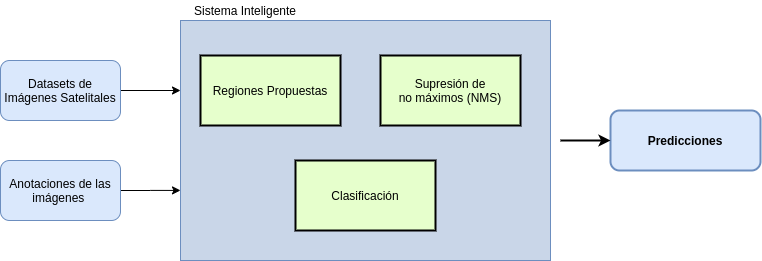
\includegraphics[height=5.5cm,keepaspectratio=true,clip=true]{imagenes/Logos/DB-Sistema.png}
  \caption{Arquitectura del Software de reconocimiento}
	\label{Fig: diagbloque}
 \end{figure}
 
Como se visualiza en el diagrama de arquitectura \ref{Fig: diagbloque}, se dispone de un bloque principal que llamamos \textit{sistema inteligente} en el comprende el calculo de \ac{rp} en base a las imagenes satelitales que recibe como entrada, el computo de NMS (sec: \ref{sub:nonmaximumsuppression}) que permite eliminar el overlapping de regiones detectadas y el bloque de clasificación integrado por todos los experimentos realizados (validación cruzada, búsqueda de hiperparametros y evaluación), en base a los datos y las anotaciones recibidas como entrada, la salida final sera la respuesta del modelo entrenado.

\section{Estructura general de la tesis }\label{sec:estructura}


La tesis se estructura de acuerdo a los siguientes capítulos: Introducción, Marco Teórico, Desarrollo del Software, Evaluación experimental , Conclusiones y trabajos a futuro, Bibliografía y Apéndice :

En el capítulo \ref{chap:marcoteorico} \textit{Marco teórico}: plantea los fundamentos e investigación que se realizaron con el fin de situar el problema dentro de limites teóricos. En este capitulo se desarrolla los conceptos claves como: ¿que es visión artificial?, los métodos que existen, diferentes algoritmos de detección que encontramos en la literatura, ¿ que entendemos por aprendizaje automático?, los campos que hacen uso de esta metodología, nombrando la importancia de las redes neuronales en el campo de reconocimiento de patrones.

El capítulo \ref{chap:tbd} \textit{Esquema de detección}: En este capítulo se describen el esquema de procesamiento (pipeline) utilizado para el desarrollo de la tesis, también se desarrollará la \textit{recolección de datos} llevada a cabo para la obtención de las imágenes.

%El \textbf{Capítulo} \ref{chap:Desarrollo} \textit{Desarrollo del Software}: En este capítulo se evalúan las diferentes herramientas utilizadas, junto con la estructura del código realizado.

El capítulo \ref{chap:evaluacion} \textit{Evaluación experimental}:  se  dividió en tres secciones principales. La primera hace referencia al los datos y procesos que se llevaron a cabo sobre las imágenes. La segunda parte se describe como se extrajo los datos de cada imagen para realizar el entrenamiento. En la sección final del capitulo se describen los métodos de validación utilizados y cuales fueron los resultados obtenidos.

En el capítulo \ref{chap:conclusiones} \textit{Conclusiones y trabajo a futuro}: se plantea las conclusiones sacadas de la investigación y experimentación además de los posibles trabajo a futuro partiendo de lo realizado.

Capítulo \textit{Bibliografía}: Se enuncian las diferentes fuentes consultadas para el desarrollo de la tesis.

Para finalizar tenemos el capítulo \ref{chap:anexo} Apéndice}: describe algunos procesos realizados para el desarrollo de la tesis como por ejemplo: instalación de librerías, desarrollo de códigos utilizados y diagramas.

\chapter{Marco Teórico} \label{chap:marcoteorico}

En el siguiente capitulo se pondrá al alcance del lector las bases teóricas y los conocimientos necesarios para poder entender las diferentes terminologías utilizadas en el trabajo de investigación realizado.

Se tratará de dar un enfoque simplificado de temas como: ¿que es el sensado remoto?, ¿que es el Aprendizaje Automático?, descripción y desarrollo de Algoritmos de optimización, validación de modelos, Computer Vision.

Para finalizar se expondrá la arquitectura, entrenamiento y reconocimiento de objetos a través de  redes neuronales convolucionales y clasificadores.

\section{Sensado Remoto}\label{sec:sensadoremoto}

En esta sección desarrollaremos el principal enfoque de este trabajo que son las imágenes satelitales; como se forman, rangos de bandas, instrumentos utilizados y datos con los cual se trabaja.

\subsection{Teledetección}\label{sub:teledeteccion}

Para comenzar a introducir el concepto de imagen satelital debemos saber como esta formada la misma, es por esto que vamos a desarrollar el concepto de \textit{teledetección}.

La teledeteccion o sensado remoto tambien llamado es el proceso que nos permite obtener una imagen de la superficie terrestre de forma remota, es decir sin estar en contacto con ella. Una imagen satelital es una representación de estos datos reflejados por la superficie terrestre que son captadas por un sensor que se encuentran a bordo de un satélite artificial (ver fig \ref{Fig:teledeteccion}).

La teledeteccion no es mas que la detección de propiedades relevantes del entorno; esta capacidad no es despreciable, nos permite desarrollar aplicaciones practicas con un impacto cada ves mayor \citep{percepcion}. 

En general la teledetección es la medición de energía emanada de la superficie terrestre. Existen diferentes fuentes de energía; si la fuente de energía es el sol entonces lo llamamos \textit{teledetección pasiva}, si la energía medida no es emitida por el Sol, es decir es emitida por un sensor, llamamos \textit{teledetección activa}, como por ejemplo los sensores de radar que funcionan en el rango de microondas.

Los componentes básicos de un sistema de teledetección incluye lo siguiente \citep{chuvieco}:
\begin{itemize}
\item \textit{Fuente de energia}: es la radiación electromagnética que capta el sensor; como mencionamos anteriormente puede tratarse de una fuente pasiva o activa.

\item \textit{Cubierta terrestre}: rasgos naturales o realizados por el hombre, ejemplo construcciones, que refleja el sensor.

\item \textit{Sistema Sensor}: esta compuesto por, cámaras, radar, etc; y la plataforma en la que esta puesto (satélite, avión, globo);  capta la energía proveniente de la tierra y la almacena o envía al sistema de recepción.

\item \textit{Sistema de Recepción}: sistema encargado de recibir la información proveniente del sensor y almacenar en un formato apropiado para luego ser distribuido a los usuarios.

\item \textit{Interprete}: encargado de manipular los datos de acuerdo a la temática de interes (agricultura, catastro, etc), es decir aplica diferentes niveles de procesamiento sobre los datos crudos obtenidos por el sensor.

\item \textit{Usuario Final}: es el consumidor final de la imagen adquirida.
\end{itemize}

\begin{figure}[H] \centering
  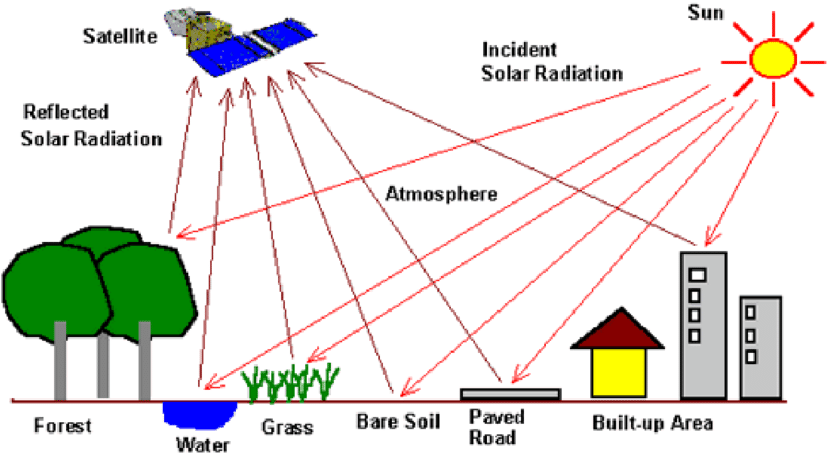
\includegraphics[height=8cm,keepaspectratio=true,clip=true]{imagenes/MarcoTeorico/teledeteccion.png}
  \caption{Sensado Remoto. Navarrete, Edison, Laubacher, Gerard}\label{Fig:teledeteccion}
\end{figure}

\subsubsection{Tipos de Sensores}
\begin{itemize}
\item \textbf{sensores pasivos}: son aquellos que reciben las señales emitidas naturalmente que fueron reflejadas por los objetos. Estas señales son a partir de la radiación solar natural. Este tipo de sensores son  usados mayormente en aplicaciones de evaluación de recursos naturales. Ejemplo: ASTER, MODIS, VIIRS, LandSat.

\item \textbf{sensores activos}: son aquellos que emiten radiación dirigida hacia un objetivo especifico, esta radiación reflejada del objeto es detectada y medida por el sensor. Ejemplo: Radar, Sonar.
\end{itemize}

\subsubsection{Espectro electromagnético}

El espectro electromagnético se denomina al conjunto de todas las longitudes de onda \citep{chuvieco}. Las ondas electromagnéticas cubren una amplia gama de frecuencias o de longitudes de ondas y pueden clasificarse según su principal fuente de producción. 
Las regiones utilizadas para la observación remota de la tierra son:
\begin{itemize}
\item Espectro visible (0.4 - 0.7 µm): rango de frecuencias del ojo humano; máxima radiación solar. Subdividido en tres bandas: Rojo (0.6 - 0.7 µm), Verde (0.5 - 0.6 µm) y Azul (0.4 - 0.5 µm).

\item Infrarrojo cercano (0.7 - 1.1 µm): denominado IR fotográfico o reflejado; energía solar que reflejan los cuerpos. Comportamiento similar al espectro visible.

\item Infrarrojo medio (1.1 – 8 µm): se entremezclan radiación solar y emisión; la atmósfera afecta sensiblemente: aprovechado para medir concentraciones de vapor de agua, ozono, aerosoles, etc.

\item Infrarrojo térmico (8 - 14 µm): radiaciones emitidas por los propios cuerpos; se puede determinar la Temperatura de un cuerpo (IRtérmico). Se puede disponer de imágenes a cualquier hora del día.

\item Microondas (1mm-1m): Interés creciente de la Teledetección en esta banda; las perturbaciones atmosféricas son menores y es transparente a las nubes. Se suelen utilizar sensores activos. 

\end{itemize}

\begin{figure}[H] \centering
  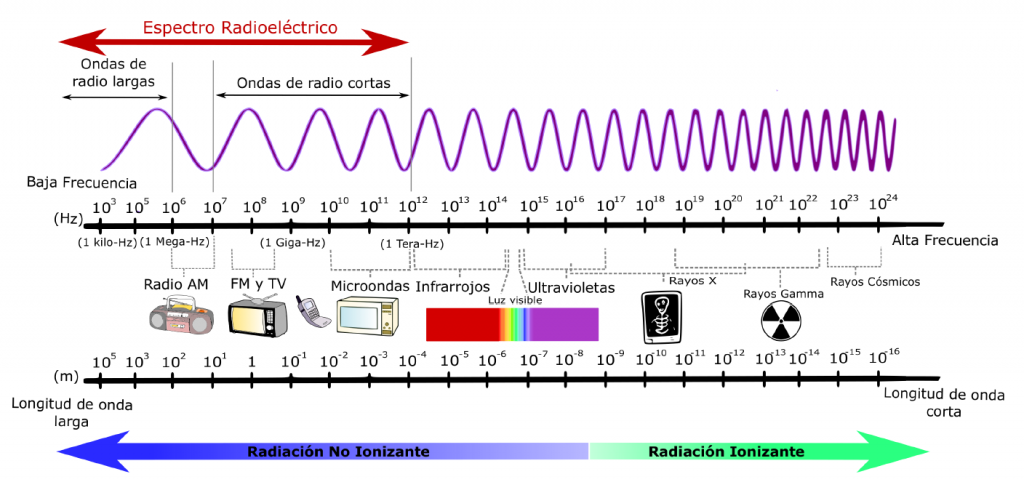
\includegraphics[height=8cm,keepaspectratio=true,clip=true]{imagenes/MarcoTeorico/espectro-electro.png}
  \caption{Espectro electromagnético \citep{https://iie.fing.edu.uy/proyectos/esopo/eem/}}\label{Fig:espectro-electromagnetico}
\end{figure}


\subsubsection{Resolución}
Unas de las características de los sensores son el tipo de imagen que proporciona; estas características vienen definidas por el timpo de resolución. Estas resoluciones la podemos definir de la siguiente manera:

\begin{itemize}
\item \textbf{Resolución Espacial}: distancia que corresponde a la unidad mínima de información incluida en un píxel. A menor tamaño de píxel mayor sera la resolución espacial, esto quiere decir que el sensor tendrá mayor detalle de los objetos.

\begin{figure}[H] \centering
  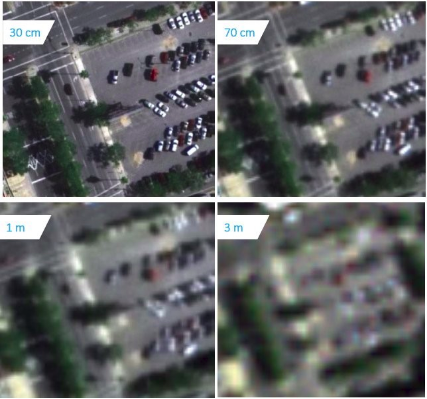
\includegraphics[height=8cm,keepaspectratio=true,clip=true]{imagenes/MarcoTeorico/resolucion.png}
  \caption{Resolución espacial \citep{https://iie.fing.edu.uy/proyectos/esopo/eem/}}\label{Fig:resolucion-esp}
\end{figure}

\item \textbf{Resolución Espectral}: la resolución espectral especifica el numero y la anchura de las badas espectrales que puede ser discrimidadas por el sensor.
\begin{figure}[H] \centering
  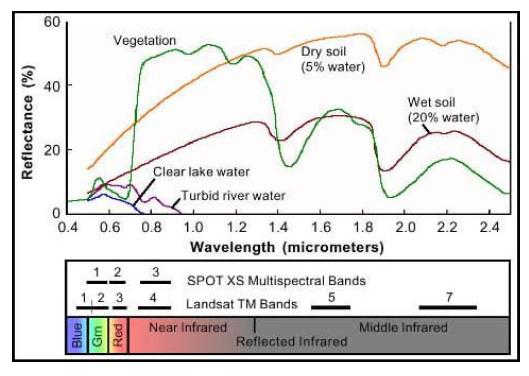
\includegraphics[height=8cm,keepaspectratio=true,clip=true]{imagenes/MarcoTeorico/resolucion_espectral.jpg}
  \caption{Resolución espectral \citep{http://laotraopinion.net/wp-content/uploads/poder-de-resolucion-espectral.jpg}}\label{Fig:resolucion-espectral}
\end{figure}

\item \textbf{Resolución Radiometrica}: indica el numero de bits utilizados para expresar los datos recogidos por el sensor. Mayormente cuando es mas grande el número de niveles mayor es el detalle con la cual se podrá expresar dicha información. Ejemplo los sensores Landsat (5 y 7) utilizan 8 bits lo que da 2**8= 256 niveles de energía que pueden ser captados.
\begin{figure}[H] \centering
  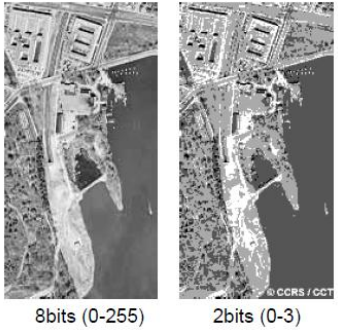
\includegraphics[height=8cm,keepaspectratio=true,clip=true]{imagenes/MarcoTeorico/resolucion_radiometrica.png}
  \caption{Resolución radiometrica}\label{Fig:resolucion-radiometrica}
\end{figure}

\item \textbf{Resolución temporal}: es el tiempo necesario que tarda el satélite en volver a visitar la misma zona de la Tierra; es decir la periodicidad con la que éste adquiere la misma imagen. Este ciclo de cobertura esta en función de el tipo de orbita de la plataforma así como del sensor. Alta resolución temporal (< 1 día - 3 días), media resolución temporal (4 - 16 días), baja resolución temporal (> 16 días).

\end{itemize}

\subsubsection{Imagen Satelital}
Una imagen satelital esta compuesta por diferentes matrices de las cuales cada celda representa un píxel; la dimensiones de este depende del tipo de resolución espacial como se mencionó anteriormente. Los sensores almacenan la raciación electromagnetica proveniente de distintas coberturas y las almacena en el píxel de acuerdo a los intervalos de onda correspondiente de cada sensor. Esta energia electromagnética se representa en cada píxel por un valor digital llamado Nivel Digital (ND), la cantidad de ND que se podrá representar depende de la resolución radiometrica.

La asignación de colores más conocido por los usuarios es el \textit{falso color} (R=Red (rojo); G=Green (verde); B=Blue (azul)), la cual asigna el color azul a la banda del verde, el color verde a la banda del rojo y el color rojo a la banda del infrarrojo cercano. 

La información obtenida de diferentes combinaciones de bandas depende del objeto de estudio que se esta llevando a cabo.

%https://acolita.com/wp-content/uploads/2018/01/Teledeteccion_espacial_ArcGeek.pdf
%https://mundosigs.wordpress.com/2016/03/07/que-son-los-sensores-remotos/
%https://www.slideshare.net/noldinn/fundamentos-deteledeteccionemiliochuvieco

\section{Aprendizaje Automático}

\subsection{Machine Learning}
\ac{ml} como se mencionó en la primera sección, es una rama de la inteligencia artificial que tiene como objetivo desarrollar técnicas que ayuden a las computadoras a aprender determinado comportamiento, generalizando, a partir de los datos de entrada. Un algoritmo de \ac{ml} es aquel que permite aprender determinado comportamiento a partir de los datos. \ac{ml} nos permite abordar tareas que son muy difíciles de resolver con programas escritos y diseñados por seres humanos.

"Se dice que un programa de computadora aprende de la experiencia E con respecto a algun tipo de tareas T y la medida de rendimiento P, si su desempeño en tareas en T, medido por P, mejora con la experiencia E." \citep{Tom michell}

Existen una gran cantidad de problemas que caen dentro de este tipo de rama, de las cuales podemos nombrar:

\begin{itemize}
\item \textit{Problemas de Regresión}: Este tipo de problema se pide que la computadora prediga un valor numérico dada alguna entrada. Los ejemplos que podemos citar son: fijar el precio de una casa a partir de las característica de la misma (cantidad de habitaciones, baños, etc), predecir el valor de la bolsa a partir del comportamiento de la bolsa en el tiempo pasado, entre otros.

\begin{figure}[H] \centering
  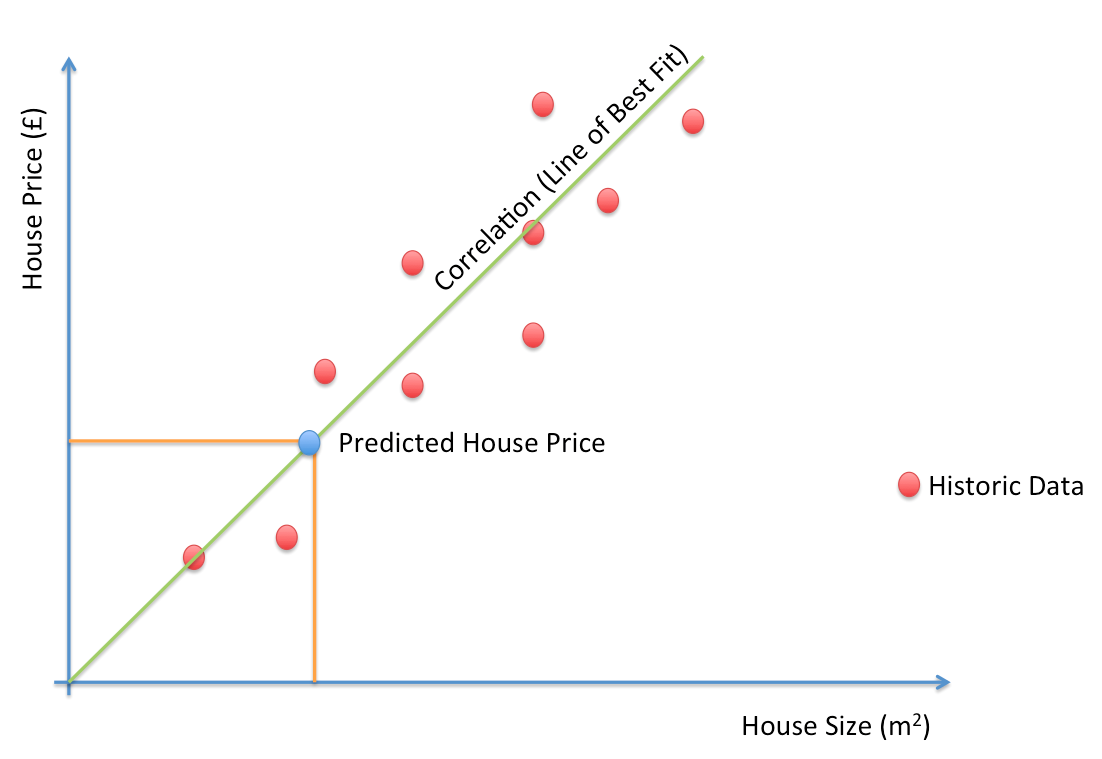
\includegraphics[height=8cm,keepaspectratio=true,clip=true]{imagenes/MarcoTeorico/regression_linear.png}
  \caption{Ejemplo Regresión (precio de una casa)}\label{Fig:regression}
\end{figure}

\item \textit{Problemas de Clasificación}: En un problema de clasificación, estamos tratando de predecir los resultados en una
salida discreta. En otras palabras, estamos tratando de asignar variables de entrada en categorías discretas. Algunos de los ejemplos son: clasificar perros o gatos determinando a que clase pertenece la imagen, evaluar si un email pertenece a la categoría "spam" o "no spam", entre otros.

\begin{figure}[H] \centering
  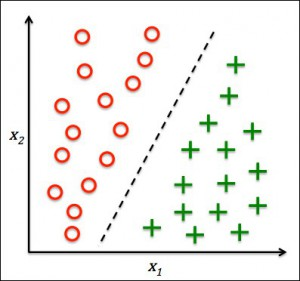
\includegraphics[height=8cm,keepaspectratio=true,clip=true]{imagenes/MarcoTeorico/classification.jpg}
  \caption{Ejemplo Clasificación}\label{Fig:clasificacion}
\end{figure}


\item \textit{Problemas de Aprendizaje no supervisado}: El aprendizaje no supervisado nos permite abordar los problemas con
poca o ninguna idea de cómo deben ser nuestros resultados. Podemos derivar la estructura de los datos donde no necesariamente conocemos el efecto de las variables. Podemos derivar esta estructura agrupando los datos basados en relaciones entre las variables en los datos. Con el aprendizaje no supervisado no hay una retroalimentación basada en los resultados de la predicción. El objetivo de problemas de aprendizaje no supervisados puede ser descubrir grupos de ejemplos similares dentro de los datos, donde se denomina agrupación (clustering), o determinar la distribución de datos dentro del espacio de entrada, conocida como estimación de densidad (density estimación), o proyectar los datos desde un espacio de nivel dimensional alto hasta dos o tres dimensiones con propósitos de visualización (Bishop, 2006).

\begin{figure}[H] \centering
  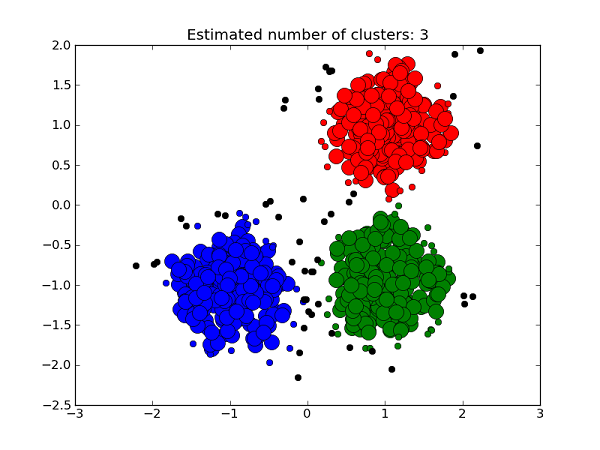
\includegraphics[height=8cm,keepaspectratio=true,clip=true]{imagenes/MarcoTeorico/claustering.png}
  \caption{Ejemplo aprendizaje no supervisado, claustering}\label{Fig:clauster}
\end{figure}
\end{itemize}

\subsubsection{Entrenamiento del modelo}
%https://docs.aws.amazon.com/es_es/machine-learning/latest/dg/training-ml-models.html
%clasificación supervisada metodos deduccion matematica
Entrenar un modelo de \ac{ml} consiste en proporcionar un conjunto de datos de entradas, datos de entrenamiento, de las cuales el algoritmo va a aprender. El algoritmo encuentra patrones en los datos proporcionados de entrada y genera un modelo que captura y generaliza dichos patrones para luego realizar predicciones sobre datos que no conoce.

Para poder entrenar un modelo necesitamos al menos tres cosas especificas:
\begin{enumerate}
\item \textbf{Datos de entrada}: determinar cuales son los ejemplos de entrada del algoritmo, el objetivo es crear un modelo que generalice los nuevos datos; para esto los datos de entrada deben ser representativo del mundo real. Por ejemplo para una tarea de clasificación entre perros y gatos los datos de entrada deben ser imágenes que pertenezcan a las categorías mencionadas; para resolver un problema de reconocimiento de voz los datos de entrada deben ser audios de personas hablando.

\item \textbf{Salida esperada}: para cada valor de entrada debemos etiquetar a que clase pertenece es decir, para un problema de clasificación entre perros y gatos debemos tener etiquetada cada imagen para saber a que clase pertenece la imagen; para un ejemplo de reconocimiento de voz cada audio debe tener una transcripción del mismo.

\item \textbf{Evaluación de las predicciones}: calcular y evaluar métricas con los resultados de la predicciones obtenidas por los modelo, es decir, determinar la distancia entre la salida esperada y los valores predichos.
\end{enumerate}

Como se desarrollo anteriormente el proceso de entrenamiento tiene: variables de entrada (x) y una variable de salida (Y); que a través de un algoritmo de aprendizaje obtenemos la siguiente relación entre estas variables como vemos a continuación.


\begin{eqnarray}
 f:X \longrightarrow Y\\
 \mbox{Training}:\qquad \{(x^i, y^i) \in X\; x\; Y \} _i=1...n\\
 \mbox{El objetivo es encontrar}\; f\; \mbox{tal que:}\qquad f(x)\approx y
\end{eqnarray}

Considerando el siguiente ejemplo, dada las cordenadas (x,y) como se muestra en la siguiente figura \ref{Fig: ejemplo-1}, se muestran dos clases, puntos de color negro y otra blanca.
\begin{figure}[H] \centering
  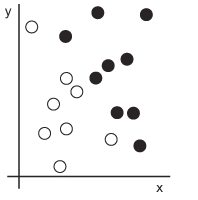
\includegraphics[height=4cm,keepaspectratio=true,clip=true]{imagenes/MarcoTeorico/sample.png}
  \caption{Ejemplo entrenamiento}\label{Fig:ejemplo-1}
\end{figure}

La idea principal de desarrollar un modelo; es crear un algoritmo que a partir de datos encuentre automáticamente una frontera, clasifique, por ejemplo encuentre una frontera entre los puntos negros y los puntos blancos.

Como se puede ver en la figura siguiente \ref{Fig:ejemplo-2}, se muestra la fontera de separación creada por el algoritmo entrenado.
\begin{figure}[H] \centering
  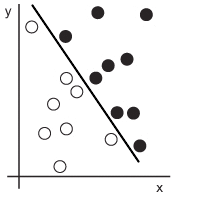
\includegraphics[height=4cm,keepaspectratio=true,clip=true]{imagenes/MarcoTeorico/sample-fit-1.png}
  \caption{Entrenamiento}\label{Fig:ejemplo-2}
\end{figure}

De esta manera cuando se pase un elemento que nunca vio puede determinar en cual de los dos espacios creado por el modelo cae este nuevo dato; en este caso estamos hablando en un algortimo de clasificación.

\subsubsection*{Ejemplo: Regresión Lineal}
%http://www.deeplearningbook.org/contents/ml.html
Una Regresión lineal es un claro ejemplo de un algoritmo de \ac{ml}; el objetivo es desarrollar un sistema que tome un vector $x \in \; $R$^n$, prediga el valor de un escalar $y \in \; $R$ $ como salida; la salida de una regresión lineal es una función lineal de la entrada.  Vamos a tomar como $\hat{y}$ el valor que nuestro modelo predice definido por:
\begin{equation}
\hat{y} = w^t * x
\end{equation}
donde $w \in \; $R$ $, siendo un vector de parámetros.
Los parámetros son valores que controlan el comportamiento del sistema,en este caso w  multiplicado por x (característica de cada datos de entrada), lo podemos ver como un conjunto de pesos que determinan como cada característica afecta a la predicción.

Si x esta multiplicado por un peso $w_i $ positivo, entonces el valor de esa característica aumenta nuestra predicción, de manera análoga si el valor $w_i $ es negativo esa característica x disminuye mi valor de predicción $\hat{y}$.
Como siguiente medida debemos medir la precisión de nuestro modelo, para realizar la medición de nuestro modelo debemos anteriormente haber separado el conjunto de datos en dos partes por un lado los datos de que se van a usar para realizar el entrenamiento y por otro los datos que serán utilizados para medir la precisión del modelo, llamado conjunto de test.

Una de las maneras de medir nuestra precisión del modelo con nuestro conjunto de test es computando el error cuadrado medio, dado por la siguiente ecuación:
\begin{equation}\label{eqn:mse} 
MSE_{test} = \frac{1}{n}\sum_{i}(\hat{y}^(test)- y^(test))^2
\end{equation}

Como se puede ver a partir del calculo anterior el error decremento a 0 cuando $\hat{y}$ es igual a $y$. Para entrenar un modelo de \ac{ml} necesitamos realizar un algoritmo que en cada iteración mejore los valores de los pesos de manera de reducir el error; en la sección siguiente se desarrollará mas en detalle.

Decimos que una hipótesis generaliza bien, cuando predice correctamente con entradas no conocidas.

\subsubsection{Función de Costo}
Existen diferentes maneras de que una algoritmo aprenda los parámetros de un modelo, este proceso de aprendizaje es posible minimizando la función de costo. Una función de costo es una medida del cuán erróneo es el modelo que estamos entrenando en términos a la capacidad de estimar la relación entre $X $ e $y $. Esto se lo puede expresar como la diferencia o distancia entre el valor predicho y el actual valor.

Como se menciono anteriormente el objetivo de un modelo de \ac{ml} es encontrar los valores que minimicen la función de costo.Una función de costo toma un conjunto de datos y retorna un valor llamado error costo (\textit{loss cost} su traducción en ingles). Existen diferentes tipos de funciones de costo que podemos usar; una de las mas comunes usada es \textbf{mean square error}, MSE, visto en \ref{eqn:mse}, en este caso determina la distancia o simplemente la diferencia entre el dato y el predictor $(x_i - y_i) $ ver figura: \ref{Fig:mse}.
\begin{figure}[H] \centering
  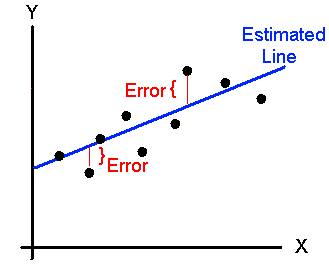
\includegraphics[height=4cm,keepaspectratio=true,clip=true]{imagenes/MarcoTeorico/mse-cost.png}
  \caption{Mean Square Error }\label{Fig:mse}
  %http://wiki.fast.ai/images/5/55/Linear_line_w_cost_function.png
\end{figure}

Dado un punto de datos $(x_i,y_i) $, donde $x_i $ es el conjunto de característica (por ejemplo pisos, dormitorios, etc) que el modelo usa para realizar la predicción, $y_i $ es la etiqueta del ejemplo (por ejemplo precio de la casa) e $y(x_i)$ es la la función de predicción; el error esta dado por la siguiente formula:
\begin{equation}\label{eqn:error-mse}
e = (y(x_i) - y_i)^2
\end{equation} 
A partir del calculo anterior podemos generalizar y tomar el promedio sobre todo los punto de datos de la siguiente manera:
\begin{equation}
MSE =  \frac{1}{n}\sum_{i}(y_i - y(x_i))^2
\end{equation}
% NOTA: SE DEBE PONER MAS FUNCIONES DE COSTO RMSE?

Existen en la actualidad diversas funciones de costo que nos permite calcular el error del modelo; entre ellas estan: Quadratic cost, Cross-entropy cost, Exponentional cost, Hellinger distance, Kullback–Leibler divergence, entre otras.

%https://stats.stackexchange.com/questions/154879/a-list-of-cost-functions-used-in-neural-networks-alongside-applications

\subsubsection{Algoritmos de Optimización} 
%https://hackernoon.com/gradient-descent-aynk-7cbe95a778da
%https://stxlearning.com/2018/03/25/optimizacion-deep-learning-y-complejidad-computacional/
En modelos de \ac{ml} debemos encontrar aquellos parámetros que minimizan la función de costo como se menciono previamente, este es un problema de optimización ya que si encontramos la solución podemos encontrar esos parámetros que disminuyen el error.

En la mayoría de los algoritmos de \ac{ml} deben aprender mas de un parámetro, en algunos casos hasta decenas de millones de parámetros; es por esto que todos los algoritmos  son métodos de optimización ya que se busca aprender los parámetros de manera eficiente. La estrategia mas típica para problemas de optimización son los llamados métodos de descenso; dentro de estos se encuentran: descenso de gradiente, descenso de gradiente estocástico y método de Newton Rawson de 2 orden.

\subsubsection*{Descenso de gradiente}\label{sub:gradient-desc}
Para encontrar el mínimo valor para grandes dimensiones de datos el algoritmo mas utilizado es el llamado \textbf{Descenso de Gradiente} (\textit{gradient descent} en ingles). El descenso de gradiente es un algoritmo de optimización que busca encontrar el mínimo local o global de una función convexa.  En \ac{ml} usamos descenso de gradiente para encontrar los parámetros de nuestro modelo que mejor definen nuestro conjunto de entrenamiento.

Este algoritmo permite que el modelo aprenda el gradiente o la dirección que el modelo debe seguir para reducir el error; en cada iteración gradualmente converge hacia un mínimo optimizando los valores $w_i $ que minimizan la función de costo. $$\min_{w} f(w)$$

Esto quiere decir que queremos encontrar los parámetros $w$ que minimicen la diferencia entre las salidas $Y$ y las producidas por el modelo dependiente de $w$. Entre menor  diferencia mejor aproximación a la salida $Y$. 

\begin{figure}[H] \centering
  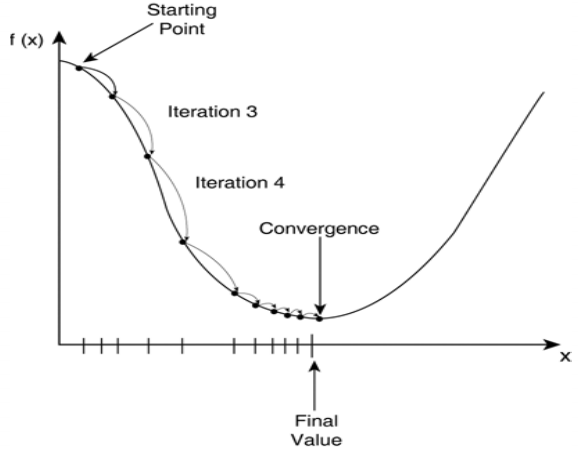
\includegraphics[height=6cm,keepaspectratio=true,clip=true]{imagenes/MarcoTeorico/gradient-descent.png}
  \caption{Gradient Descent }\label{Fig:gradient-descent}
\end{figure}


%Gradiente extraido de :https://www.cs.huji.ac.il/~shais/UnderstandingMachineLearning/understanding-machine-learning-theory-algorithms.pdf
El gradiente de una función diferenciable $ f: R^d \longrightarrow R $ en $\textbf{w}$, denotado $ \nabla f(w) $ vector de derivadas parciales de la función $f$ es decir:
\begin{equation}
\nabla f(x) = (\frac{\partial f(\textbf{w})}{\partial w[1]},....., \frac{\partial f(\textbf{w})}{\partial w[d]})
\end{equation}

Descenso de gradiente es un algoritmo iterativo; comenzamos con un valor inicial de $\textbf{w}$ (el valor 0 por ejemplo), luego en cada iteración damos un paso en la dirección negativa del gradiente en el punto actual. Es decir, el paso de actualización es:
\begin{equation}
\textbf{w}^{(t-1)} = \textbf{w}^{(t)} - n \nabla f(\textbf{w}^{(t)})
\end{equation}
En el cual $n > 0$, dado que el gradiente apunta a la dirección del mayor índice de $f$ alrededor $w^{(t)}$, el algoritmo va en sentido opuesto disminuyendo el valor de la función. Luego de T iteraciones se genera un vector promedio dado por: $ \hat{w} = \frac{1}{T} \sum_{t=1}^T w^{(t)}$; la salida también puede ser el vector con mayor  $ argmin_{t \in [T]} f(w^{(t)}) $.


En dónde $\hat{w}$ es una nueva posición de los parámetros que se acercan más al mínimo buscado, es decir que hacen que $f(w^{(t)})$ aproxime mejor a $Y$ .

% PONEMOS BACKPROPAGATION, LEARNING RATE

%http://ruder.io/optimizing-gradient-descent/
%https://turing.iimas.unam.mx/~ivanvladimir/posts/gradient_descent/

\subsubsection{Validación de Modelos}
%Validación de Modelos (overfitting, underfitting)


\subsection{Computer Vision}

\subsection{Ajuste de Modelos}

\subsection{Redes Convolucionales}

\subsection{Regions Proposal}

\subsection{Clasificadores}








%\chapter{Estado del Arte} \label{chap:estadodelarte}


En este capítulo vamos a describir las diversas investigaciones y trabajos realizados con imágenes satelitales hasta la fecha. Se pondrá a disposición del lector como se utilizaron técnicas de  Computer Vision y Machine Learning sobre imágenes satelitales.


\section{Aplicaciones en el ámbito espacial}\label{sec:estadodelacuestion}

Las aplicaciones de visión artificial en el ámbito espacial son cada ves mas utilizadas, desde el estudio de un área determinada hasta implementaciones echas a bordo de un satélite artificial. Este avance se dio gracias a diversos factores en el campo de la informática; en primer lugar la creciente capacidad de computo, con procesadores de mayor rendimiento y el auge de las GPU (unidad de procesamiento grafico). En segundo lugar la aparición de algoritmos y frameworks mas eficiente en el uso de reconocimiento de patrones; de los que podemos nombrar el uso de \ac{cnn}. 

Otro factor que no podemos dejar de nombrar son la aparición de UAVs, esto permitió utilizar Computer Vision sobre imágenes de mayor tamaño. La presencia en el mercado de pequeños UAVs de bajo costo con capacidad para portar pequeñas cámaras de vídeo de alta resolución y de realizar despegue vertical con posibilidad de movimiento en cualquier dirección del espacio, hace posible abordar nuevos retos en el campo de la detección y seguimiento de determinadas situaciones de la realidad \citep{Lanillos}.

Actualmente en el campo de reconocimiento de patrones sobre imágenes satelitales se pude ver que la mayoría de los trabajos que se realizaron en el área espacial han sido aplicado en tierra; gran parte de estos trabajos se basan en estudiar las característica del terreno. Estas aplicaciones son cada vez mas explotada no solo por agencias espaciales sino por entidades educativas, publicas y privadas. 

Para empezar vamos a comenzar citando el siguiente trabajo realizado por \citep{Cheang}; en este articulo se describe el uso de técnicas de reconocimiento de patrones usando aprendizaje supervisado. El método para la extracción y clasificación de los datos utilizado se baso en dos enfoques; por un lado se utilizaron técnicas de \textit{sliding window} para la obtención de regiones candidatas, por otro se aplicaron redes neuronales profundas, \ac{dl}, método muy utilizado para el reconocimiento de objeto en una imagen. Otro ejemplo encontrado en la literatura aplicando  \textit{aprendizaje no supervisado} es para la clasificación del uso de la tierra a partir de imágenes satelitales multi-temporales, en este paper \citep{pnn}, se utilizo imágenes del satélite LANSAT y SPOT usando redes neuronales probabilística, estas técnicas realizan un agrupamiento de datos, \textit{clusters}, y realizan la clasificación creando las fronteras entre los diferentes \textit{clusters} de datos para su posterior reconocimiento.

En el blog titulado \textit{Una imagen vale más que mil palabras}, los autores destacan el beneficio de aplicar procesamiento en imágenes para la toma de decisiones que agregan valor a su negocio. En este articulo describen la posibilidad de conocer el historial de inundaciones de una region rural aplicando técnicas \ac{ml} sobre imágenes satelitales\footnote{Fuente:http://www.7puentes.com/blog/2017/12/11/agtech-imagenes-satelitales-una-imagen-vale-mas-que-mil-palabras/}.

El uso de \ac{va} permite crear mapas urbanos a partir de imágenes satelitales como menciona en el articulo \citep{detectionHOG}; en el mismo usa \ac{va} para crearon mapas urbanos que determinan cambios temporales en una determinada región geográfica. En este trabajo los autores proponen dos módulos para el desarrollo; por un lado usar \textit{HOG}, histograma de gradientes orientados, para la extracción de características en la imagen y \textit{Local binary patterns (LBP)}, patrones binarios locales, como método descriptor de característica; por ultimo para clasifica la imagen utilizaron técnicas SVM (ver:\ref{sub:svm}). 

\cite{usman} en su articulo describe la extracción de características de una imagen satelital aplicando métodos de  detección de bordes, \textit{edges proposal}, para el 
reconocimiento de límites catastrales.

Como podemos se puede observar en los trabajos citados anteriormente, son diversas las investigaciones realizadas sobre imágenes satelitales utilizando algoritmos entrenados para reconocer patrones de interés. En el área espacial uno de los principales problemas es la limitación de energía, esto hace que el poder de computo sea mucho menor en relación a lo que podemos utilizar en tierra, por este motivo son mucho menor los ejemplos que podemos encontrar en la literatura. Sin embargo en la actualidad existen diferentes aplicaciones que están siendo utilizadas usando este tipo de técnicas de las cuales nombraremos a continuación.

Unos de los ejemplos destacados de investigaciones en\ac{va} en vuelo es el realizado por el \textit{Dr.Tweddle} que en su trabajo titulado, \textit{Computer Vision Based Navigation for Spacecraft Proximity Operations}, estudia y detalla el uso de \ac{va} para realizar una navegación autónoma en satélites. En esta tesis destaca el proyecto de un Nanosatélite, CubeSat, de la \ac{nasa} llamado , Synchronize Position Hold Engage and Reorient Experimental Satellite (\textit{SPHERES}), que dispone de un modo experimental del uso de tecnología de visión artificial, en este paper destaca la ventaja que nos pude dar del uso de \ac{va} en relación a otra tecnología de sensado \citep{Brent}.

En la actualidad existen aplicaciones desarrolladas que utilizan algoritmos de \ac{va} en un satélite artificial; la mayoría de estas aplicaciones utilizan técnicas orientadas al aprendizaje autónomo, esto se debe a las grandes distancias que existen entre la tierra y el espacio es por esto que es necesario lograr mayor autonomía en la toma de decisiones; un ejemplo de lo mencionado es el \textit{Mars Rover}, robot desarrollado para la exploración de la superficie de Marte. El \textit{Mars Rover} crea mapas de entorno de la superficie para determinar su ubicación y predecir los diferentes obstáculos que hay en su entorno \citep{RoverMars}. Este robot utiliza  diversas cámaras que aplicando técnicas de \ac{va}  permite crear mapas del entorno y realizar la predicciones de su ruta. De la misma manera el trabajo realizados  por \ac{nasa}  destaca el uso de reconocimiento de patrones en un robot por medio de diferentes cámaras que captan la profundidad y posición del objeto\footnote{Fuente: 
http://blog.infaimon.com/robots-guiados-por-vision-artificial-para-el-espacio-robos-guiados-por-visao-artificial-para-o-espaco/}. En el informe se menciona el uso de \ac{va} para brindar soporte a los astronauta en la Estación Espacial Internacional (ISS). 

Siguiendo la misma linea de investigación podemos nombrar el proyecto \textit{Docking and Capture of Satellites through computer vision}, ASIROV: Acoplamiento y Agarre de Satélites mediante Sistemas Robóticos basado en Visión \footnote{Fuente: https://goo.gl/w7iayv}, desarrollado para atracar y capturar satélites espaciales; este sistema se basa  en tecnologías de \ac{va} para guiar de forma autónoma un vehículo espacial.


Usar técnicas de \ac{va} implica lograr que el satélite tenga mayor autonomía, en el articulo realizado por \cite{Kouyama}, aplica esta tecnología para determinar la actitud y órbita del satélite basado en los datos adquiridos por los sensores del mismo; en el articulo los autores describen que para pequeños satélites,CubeSat, tienen una carga útil limitada y sus actitudes a veces son difíciles de determinar a partir de los pocos sensores que contiene a bordo por sí solos. Estas actitudes incorrectas conducen a proyecciones y mediciones inexactas que requieren corrección de pos-procesamiento en tierra. En el estudio proponen un esquema automatizado y robusto que deriva la actitud del satélite a partir de sus imágenes de observación y de la posición de satélite conocida, combinando características de tierra de una imagen observada y de imágenes registradas. El esquema combina algoritmos de \ac{va} (es decir, detección de características y validaciones robustas) y restricciones geométricas de la observación por satélite.

\cite{Huggins} en su trabajo titulado \textit{Computer Vision Localization Based on Pseudo-Satellites} propone usar técnicas de \ac{va} para la localización y orientación de un CubeSat para complementar la navegación, el estudio se enfoca en  aumentar la capacidad de los GPS utilizando \ac{va}. El autor siguiere crear una red de nodos en el cual un grupo de nodos poseen GPS para calcular su posición y el otro grupo a partir del uso de la posición de la cámara y usando técnicas de  \ac{va}  utilizar la posición del primer grupo para calcular la suya intercambiando información de los datos y calculando la distancia y orientación de la cámara \citep{Huggins}.

Como vimos existen en la actualidad estudios y aplicaciones realizadas ya sea en vuelo o en tierra que utilizan algoritmos de reconocimiento de patrones, por lo que la tendencia vista en los últimos tiempo es muy alentadora y nos abre una nueva forma de mirar al espacio y enfocar nuestro desarrollo a esta área, como podemos ver en el gráfico siguiente \ref{Fig: scopus1}. 

\begin{figure}[h]
 \centering
  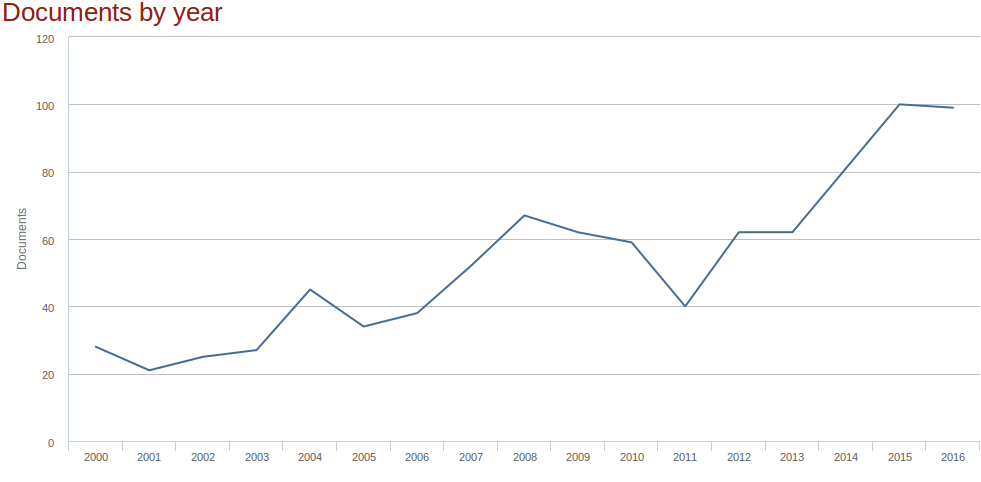
\includegraphics[height=7cm,keepaspectratio=true,clip=true]{imagenes/Logos/scopus.png}
  \caption{Extraído de Scopus.com}
	\label{Fig: scopus1}
\end{figure}
Los datos que muestran la siguiente figura \ref{Fig: scopus2} han sido relevados desde el año 2000 hasta la fecha.

\begin{figure}[h]
 \centering
  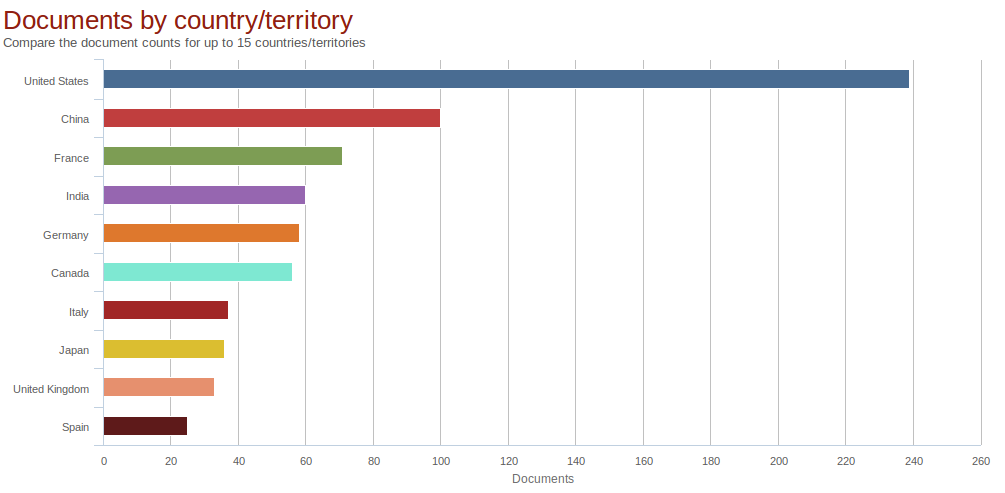
\includegraphics[height=7cm,keepaspectratio=true,clip=true]{imagenes/Logos/scopus2.png}
  \caption{Extraído de Scopus.com}
	\label{Fig: scopus2}
\end{figure}



%\chapter{Metodología}\label{chap:metodologia}
En este capítulo se detallan los diferentes procesos en el desarrollo del software que se llevaron a cabo para la realización de la tesis, es decir cuales fueron las diversas etapas que se debió realizar y cual fue su organización.

\begin{center}
\begin{minipage}{0.8\linewidth}  \vspace{5pt} {\small
Una metodología en el desarrollo se refiere al entorno que se usa para estructurar, planificar y controlar el proceso de desarrollo de un sistema de información. Este proceso es un conjunto de actividades que conducen a la creación de un producto .}
\begin{flushright}
  \citep{sommerville}
\end{flushright}
\end{minipage}
\end{center}

El modelo utilizado para el desarrollo de esta tesis está en función de los objetivos planteados en el Capítulo \ref{chap:introduccion}. La misma se dividió en diferentes fases, siguiendo un modelo de desarrollo incremental e iterativo.

En los siguiente ítems se describirán las diferentes fases que se llevo a cabo para alcanzar el objetivo planteado en el desarrollo de la tesis:
\begin{itemize}
	\item \textbf{Fase 1: Investigación de la temática de estudio}\\
	En esta fase se realizó la búsqueda bibliográfica relacionada a la temática de estudio (visión artificial, detección de objeto, 
	Aprendizaje Profundo, Aprendizaje Automático, imágenes satelitales, librerías de desarrollo, métodos de clasificación y regresión).
	\item \textbf{Fase 2: Preparación e Instalación de entorno de Desarrollo.}\\
	En esta fase se realizó la instalación de las herramientas y librerías necesarias para el desarrollo del software; se instalaron librerías  
como(Keras, SkLearn, Python-libs, entre otras).
	\item \textbf{Fase 3: Análisis e Diseño del Software.}\\
	Se analizaron diferentes técnicas de \ac{va} y \ac{ml} para ser implementadas. En esta fase también se recopilo los \textit{datasets} (conjunto de datos) para el desarrollo.
	\item \textbf{Fase 4: Desarrollo y Evaluación de resultados.}\\
	En esta fase se realizo la evaluación experimental de los datos obtenidos, optimizando los diferentes parámetros para la obtención de un 
modelo mas eficiente.
	\item \textbf{Fase 5: Escritura de Informe y Conclusiones.}\\
	Para finalizar se realizó la escritura de la tesis además se elevaron las conclusiones del desarrollo, evaluando lineas futuras de trabajo.
\end{itemize}

% \section{Requerimientos del Software}\label{sec:requerimientos}

% En la siguiente (tabla: \ref{tab:tabladerequerimiento}), se enumeran las especificaciones de requerimiento en el desarrollo del software. 
% \begin{table}[H]
% 	\begin{center}
% 	\begin{tabular}{|c|p{9cm}|c|}\hline
% 		\rowcolor[gray]{0.9} \textbf{\large ID} & \centering \textbf{\large Requerimientos} &\textbf{\large Tipo}\\
% 		\hline
% 		0 & El sistema deberá detectar un área de interés en una imagen satelital &Funcional\\\hline
%         2 & La imágenes deberá tener las bandas TBD del espectro visible & TBD\\\hline
%         3 & El software usará técnicas de Machine Learning para el procesamiento de la imágen satelital & Funcional	\\\hline
%         4 & EL software usará técnica de Computer Vision para el procesamiento de la imágen satelital. & Funcional \\\hline
%         5 & Se deberá contar con datos de entrada para su simulación: un conjunto de imágene, datos de coordenadas de los puntos de interés & Funcional	\\\hline
%         6 & El software deberá ser implementado en un lenguaje de programación que soporte tecnología de ML y VA & TBD	\\\hline
%         7 & El software deberá ser documentado  & TBD	\\\hline
%         8 & El software medirá el tiempo de procesamiento de las técnicas a usar  & TBD	\\\hline
%        	9 & El software deberá hacer un pre-procesamiento de la imágen  &	TBD\\\hline
% 	\end{tabular}
%     \caption{Requerimientos de Software} \label{tab:tabladerequerimiento}
%     \end{center}
% \end{table}

\section{Contexto del Sistema}\label{sub:casodeuso}

En la siguiente figura (ver: \ref{Fig: diagbloque}), se muestra el diagrama de bloque del sistema, donde observamos la arquitectura general del software. 

\begin{figure}[H]
 \centering
  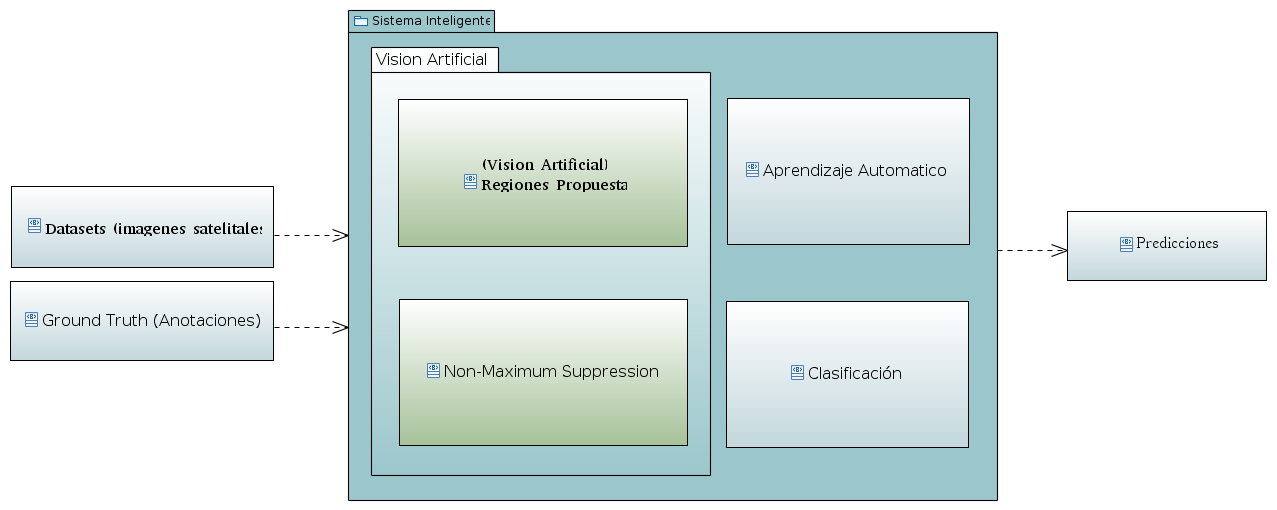
\includegraphics[height=7cm,keepaspectratio=true,clip=true]{imagenes/Logos/diagramabloque.png}
  \caption{Arquitectura del Software de reconocimiento}
	\label{Fig: diagbloque}
 \end{figure}

%\chapter{Desarrollo del Software}\label{chap:Desarrollo}
En este capítulo se describirá el lenguaje de programación utilizado para el desarrollo, las librerías utilizadas junto con el entorno de trabajo.

\section{Detalles Técnicos e Implementación}\label{sec:implementacion}
Este apartado describirá la parte técnica, herramientas y  dificultades encontradas.

\subsubsection*{Python}
Python es un lenguaje de programación de código abierto y multiparadigma que permite la programación orientada a objeto, funcional e imperativa. 
Cuenta con estructuras de datos eficientes y de alto nivel, el interprete de Python puede extenderse fácilmente  con nuevas funcionalidades y tipos 
de  datos implementados en C o C++, además cuenta con una amplia comunidad de soporte y 
documentación \footnote{Fuente:www.docs.python.org.ar/tutorial}. 

Los principales motivos por el cual se optó por este lenguaje de programación es:
\begin{itemize}
 \item Facilidad de implementación y manipulación de grandes cantidades de datos.
 \item Lenguaje muy utilizado en el ámbito laboral de \ac{ml}.
 \item Posee diversas librerías para \ac{ml} y manipulación de datos e imágenes.
\end{itemize}


\subsubsection*{OpenCV}
\ac{opencv} , es una librería de código libre que nos permite manipular imágenes de manera mas eficiente; esta librería se usa en diferentes ámbitos 
no solo académico, sino también en ámbitos comerciales, como ejemplo en sistemas de seguridad para detección de movimiento, control de procesos, 
control de calidad de alimentos, automatización de vehículos y en numerosas áreas de la ciencia como robótica, detección de objetos, reconstrucciones 
3D, realidad aumentada, etc. \footnote{Fuente: http://opencv.org/} La biblioteca \ac{opencv} puede ser usado bajo licencia BSD (Berkeley Software 
Distribution) \footnote{Fuente: https://blog.desdelinux.net/hablemos-de-la-licencia-bsd/ } para proyectos escolares o comerciales. 

Dentro del ambiente de reconocimiento de patrones es una librería muy utilizada, además es posible integrar con el lenguaje python.

\subsubsection*{Keras}

Es una interfaz de programación (API) de alto nivel para redes neuronales, escrita en python , para la manipulación y uso de modelos de \ac{dl}. 
Envuelve las eficientes bibliotecas de cálculo numérico Theano y TensorFlow y permite definir y entrenar modelos de redes neuronales en unas breves 
líneas de código \footnote{Fuente:  https://keras.io/}. Como principal inconveniente encontrado es la escasa documentación de la librería.

\subsubsection*{Scikit-Learn}\label{sub:sklearn}
Scikit-Learn es una librería de software desarrollada en Python para solucionar problemas de \ac{ml}; que comprende en intentar predecir datos 
desconocidos a partir de modelos creados. Cuenta con varios algoritmos para la solución de problemas de ,regresión, clasificación y clustering, 
incluyendo algoritmos como maquinas de soporte vectoriales, vecino mas cercano (K-NN), descenso de gradiente , entre otros\footnote{Fuente: 
http://scikit-learn.org/stable/index.html}.

Su principal ventaja es la fácil implementación y manipulación de los algoritmos contenidos en la librería.

\subsubsection*{Entorno de desarrollo}
El entorno de desarrollo utilizado fue el ID \textit{Eclipse}, herramienta de código abierto multiplataforma. La herramienta está diseñada para 
ser extendida de forma indefinida a través de \textit{plug-ins}. Sus principales características son:
\begin{itemize}
 \item Perspectivas, editores y vistas
 \item Gestión de proyectos
 \item Extensa colección de \textit{plug-ins}
\end{itemize}
El \textit{plug-ins} utilizado para el desarrollo de la tesis fue \textit{Pydev, EGit}. El principal inconveniente encontrado de esta herramienta es 
el consumo de memoria cuando se esta ejecutando, así también se presentaron inconvenientes a la hora de realizar un commit en un repositorio Git.

\subsubsection*{Control de Versiones}

Las herramientas que se utilizaron para llevar un control del versiones en el desarrollo fueron: \textit{GitHub}\footnote{Fuente: https://github.com/} 
y \textit{GitLab} \footnote{Fuente : https://about.gitlab.com/} , son software pensado en el mantenimiento de aplicaciones. El objetivo de estas 
aplicaciones gestionar los diversos cambios que se realizaron sobre los elementos de algun producto o alguna configuración del mismo; una versión, 
revisión o edición del producto, es el estado en el cual se encuentra el mismo.

Las características principales son: herramientas gráficas para ver como se trabajo en el proyecto, entorno colaborativo permitiendo a diferentes 
desarrolladores compartir sus trabajos, registro histórico de cada acción realizada en cada elemento, seguimiento de errores.

\subsubsection*{ENVI}\label{sub:enviSoft}
El software de análisis de imágenes \textit{ENVI} es utilizado por profesionales de GIS, científicos e analistas de imágenes para extraer información 
significativa de las imágenes para tomar mejores decisiones. ENVI se puede implementar y acceder desde el escritorio, en la nube y en dispositivos 
móviles y puede personalizarse a través de una API para cumplir con los requisitos específicos del proyecto \footnote{Fuente: 
http://www.harrisgeospatial.com/Learn.aspx}.

ENVI proporciona una poderosa API que permite agregar sus propios algoritmos propietarios, ampliar las herramientas y modelos existentes, automatizar 
las tareas de alta frecuencia y combinar múltiples herramientas para producir los resultados deseados.

El principal inconveniente encontrado es la instalación de herramientas adicionales para la manipulación de las imágenes como, VIIRS Toolkit. Otra 
falencia encontrada es lo poco amigable para el usuario a la hora de trabajar con imágenes.

\section{Organización y Estructura del código}\label{sec:estructuracodigo}

\textcolor{red}{ La estructura del trabajo se ha organizado en varios componentes con el objetivo hacer el código mas reutilizable. }

La estructura del directorio de trabajo es la siguiente:
\begin{itemize}
 \item \textbf{CNN}: Las funciones que contiene realizan el calculo del \textit{feature vector} a través de una red neuronal utilizando la librería 
\textit{Keras}.
 \item \textbf{ImgManipulation}: Almacena las diferentes funciones que permiten la manipulación de las imágenes de entrada 
 \item \textbf{Notacion}: Contiene diferentes clases que permiten calcular los bounding box y \ac{nms}; también contiene las funciones que almacenan 
la notaciones.
 \item \textbf{Proposal}: Contiene la clase que ejecuta regions proposal.
 \item \textbf{TensorF}:Almacena las funciones que permiten realizar el entrenamiento de los datos utilizando \textit{Scikit-Learn}.
\end{itemize}

\begin{figure}[H]
 \centering
  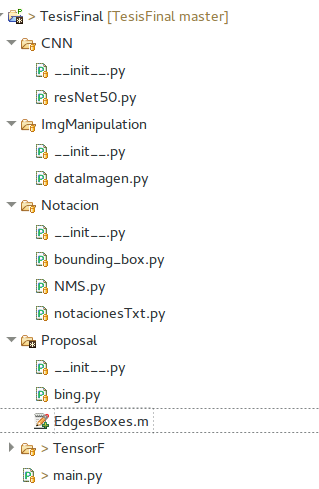
\includegraphics[height=10cm,keepaspectratio=true,clip=true]{imagenes/Logos/structureData.png}
  \caption{Estructura de directorio de trabajo}
\end{figure}

\textcolor{red}{ Para gestionar el proceso de automatización de los datos se creo un scripts principal.}

\textbf{main.py}\\
Este scripts constituye la parte principal del proceso automatizado; llamando a las diferentes clases mencionadas previamente. Las principales 
acciones que lleva a cabo son:
\begin{itemize}
 \item Lee las carpetas que contiene las imágenes junto con las anotaciones de cada una de ellas.
 \item Comprueba que exista las notaciones
 \item A cada imagen realiza el crops(recorte) correspondiente.
 \item Extrae las anotaciones de cada imagen.
 \item Llama a la clase correspondiente para calcular \textit{regions proposal}.
 \item Calcula el \textit{overlapping}, \ac{nms} para cada imagen.
 \item Calcula los \textit{feature vector}
 \item Almacena los datos en un archivo .mat
 \item Para finalizar realiza una llamada a la función para el entrenamiento.
\end{itemize}

\subsubsection*{Documentación}\label{sub:documentacion}
Para documentar el desarrollo realizado se utilizo la herramienta \textbf{\textit{Doxygen}}. Esta herramienta es un generador de documentación de fácil integración y uso en python.
%\chapter{Recolección de Datos}\label{chap:recoleccion}

En este capítulo se describirá  los pasos que se llevaron a cabo para obtener los datos de la tesis. Se  desarrollara de manera mas detallada como se obtuvo el dataset y que configuraciones de bandas se usaron para la construcción de las imágenes.


\section{Imágenes Satelitales}

Una imagen satelital se la puede definir como la representación visual de información capturada por un sensor montado en un satélite artificial (Sec:\ref{sub:imagen_satelital}). Estos sensores recogen la información reflejada por la superficie de la tierra que luego es enviada para su posterior procesamiento.

El uso de imágenes satelitales constituye una excelente herramienta para el conocimiento y monitoreo de los territorios y recursos; hoy en día disfrutamos de la oportunidad de aprovechar estas imágenes satelitales para una gran variedad de aplicaciones como: desarrollo y planificación urbana, infraestructura, recursos naturales, investigación, alerta temprana de catástrofes, asuntos militares, entre otras.

Una imagen satelital debe pasar por diferentes niveles de procesamiento dependiendo el tipo de uso que se le quiera dar, en la siguiente sección (Sec:\ref{sub:nivelesdeprocesamiento}) se desarrolla mas en detalle.

\subsection{Niveles de procesamiento}\label{sub:nivelesdeprocesamiento}

En el campo de la teledeteccion (Sec:\ref{sub:teledeteccion}) cuando hablamos de niveles de procesamiento nos referimos a los diversos procesos que son aplicados a una imagen satelital. Dependiendo de la agencia espacial existe una nomenclatura para determinar que niveles de procesamiento fueron aplicados.

En este trabajo se utilizo la nomenclatura propuesta por \ac{nasa}:
\begin{itemize}
	\item \textbf{Nivel 0}: La información científica recogida está a máxima resolución, ordenada temporalmente y con errores de transmisión, artefactos y duplicados eliminados.
 	\item \textbf{Nivel 1a}: La información esta ordenada cronológicamente y datos auxiliares como coeficientes de calibración y parámetros de referencia.
 	\item \textbf{Nivel 1b}: La información del 1a es procesada a unidades de detección, geo-refereciada.
 	\item \textbf{Nivel 2}: Variables geofísicas derivadas por ejemplo productos de concentraciones de hielo, ola de mar, etc.
 	\item \textbf{Nivel 3}: Las variables son mapeadas uniformemente en \textit{grids} espacio-temporales.
 	\item \textbf{Nivel 4}: Resultados de los análisis de los niveles anteriores
\end{itemize}


\section{Datos raw}\label{sec:datosutilizados}

Los datos utilizados para el desarrollo de los experimentos fueron descargadas por medio del catalogo  publicado en el sitio oficial de \ac{conae} \footnote{Fuente: http://catalogos.conae.gov.ar/catalogo/catalogo-de-imagenes.html} de acceso gratuito para el publico. Se debe señalar además que se trabajó con imágenes correspondiente a los años 2017 y 2018 con una ventana de tiempo desde Abril del 2017 a Marzo del 2018; estas imágenes son de naturaleza óptica con un nivel de procesamiento \textbf{1a}, de acuerdo a las nomenclaturas utilizadas en la sección (Sec:\ref{sub:nivelesdeprocesamiento}).

De acuerdo a las característica del proyecto y tomando como fundamentación lo expuesto en la sección (Sec:\ref{sec:fundamentacion}), se utilizaron imágenes que se asemejan a las características del \ac{fs} \ac{conae} detalladas en los requerimientos formales del mismo; estas imágenes fueron adquiridas por el instrumento \ac{viirs} (Sec:\ref{sub:viirs}) a bordo del satélite Suomi-NPP.


Para la realización de diversos experimentos se utilizaron en total 29 combinaciones de bandas \ref{tab:combinacion_banda}, contando con 50 imágenes por cada combinación de bandas que se realizo.


\subsection{Instrumento VIIRS}\label{sub:viirs}
El instrumento \ac{viirs} fue lanzado a bordo del satélite Suomi-NPP el 28 de octubre de 2011. Este instrumento posee 5 canales de alta resolución (I-bands), 16 canales de resolución moderada (M-bands) y un canal de baja luz (Day/Night Band, DNB).  En el siguiente cuadro se detallan las diferentes longitudes de onda y los rangos de onda de las bandas, junto con resolución geométrica apuntando a Nadir (ver tabla: \ref{tab:viirs}).
\begin{table}[H]
\begin{center}
\begin{tabular}{|c|c|c|}
\hline Banda & Rango Espectral (um) & Resolución Nadir \\\hline 
 		M1  & 0.402-0.422   & 0.742 x 0.259 \\ \hline 
		M2  & 0.436-0.454   & 0.742 x 0.259 \\ \hline 
		M3  & 0.478-0.498   & 0.742 x 0.259 \\ \hline 
		M4  & 0.545-0.565   & 0.742 x 0.259 \\ \hline 
		I1  & 0.600-0.680   & 0.371 x 0.387 \\ \hline 
		M5  & 0.662-0.682   & 0.742 x 0.259 \\ \hline 
		M6  & 0.739-0.754   & 0.742 x 0.776 \\ \hline 
		I2  & 0.846-0.885   & 0.371 x 0.387 \\ \hline 
		M7  & 0.846-0.885   & 0.742 x 0.259 \\ \hline 
		M8  & 1.230-1.250   & 0.742 x 0.776 \\ \hline 
		M9  & 1.371-1.386   & 0.742 x 0.776 \\ \hline 
		I3  & 1.580-1.640   & 0.371 x 0.387 \\ \hline 
		M10 & 1.580-1.640   & 0.742 x 0.776 \\ \hline 
		M11 & 2.225-2.275   & 0.742 x 0.776 \\ \hline 
		I4  & 3.550-3.930   & 0.371 x 0.387 \\ \hline 
		M12 & 3.660-3.840   & 0.742 x 0.776 \\ \hline 
		M13 & 3.973-4.128   & 0.742 x 0.259 \\ \hline 
		M14 & 8.400-8.700   & 0.742 x 0.776 \\ \hline 
		M15 & 10.263-11.263 & 0.742 x 0.776 \\ \hline 
		I5  & 10.500-12.400 & 0.371 x 0.387 \\ \hline 
		M16 & 11.538-12.488 & 0.742 x 0.776 \\ \hline 
\end{tabular}
\end{center}\caption{Característica de bandas,\ac{viirs} \label{tab:viirs}}
\end{table}

\subsection{Combinaciones de bandas en canales RGB}\label{sub:comb_de_banda} 
%http://www.gisandbeers.com/combinacion-de-imagenes-satelite-landsat-sentinel-rgb/

Las redes neuronales que vamos a utilizar para la construcción de esta tesis son redes neuronales pre-entrenadas (Sec:\ref{sub:cnn}), estas redes neuronales necesitan como entrada imágenes ópticas con tres canales correspondiente a \textit{RGB} (rojo, verde y azul), los canales RGB se emplean para representar distintos colores a partir de la mezcla de cada uno de estos.

Para construir el dataset de entada a la red se debió convertir los datos \textit{raw} en imágenes tomando como base los canales RGB mencionados. Las combinaciones de bandas en imágenes satelitales nos ayudan a analizar diferentes elementos dentro de la misma imagen, para esto utilizamos diversas combinaciones de bandas en cada canal RGB que que nos muestran diferentes elementos de acuerdo a la banda utilizada. El paso de cada banda por un canal RGB especifico permitirá teñir de colores los elementos que ofrezcan mayor o menor reflexión de longitudes de onda como por ejemplo, la vegetación, focos de incendios, entre otros brindando diversa fuente de información para ser explorada. 

En el siguiente cuadro  \ref{tab:combinacion_banda} se puede ver todas las combinaciones de bandas utilizadas para la construcción del dataset. El conjunto de bandas seleccionadas para los experimentos son las de resolución moderada (M-bands) \ref{tab:viirs} , que posee una resolución espacial a nadir de 750 metros.

\begin{table}[H] \begin{center}
\begin{tabular}{|c|c|}\hline 
Num & Combinación de banda\\ \hline 
1  	& 	M1-M1-M1 	\\ \hline
2  	&   M1-M3-M5	\\  \hline
3  	& 	M1-M5-M3	\\ \hline
4  	&   M3-M1-M5 	\\ \hline
5   & 	M3-M3-M3 	\\ \hline
6   & 	M3-M5-M1 	\\ \hline
7   & 	M5-M1-M3 	\\ \hline
8   & 	M5-M3-M1 	\\ \hline
9   &   M5-M5-M5  	\\ \hline
10  &	M7-M7-M7   	\\ \hline
11  & 	M9-M9-M9   	\\ \hline
12  & 	M11-M7-M9  	\\ \hline
13  & 	M11-M9-M7  	\\ \hline
14  &  	M7-M11-M9  	\\ \hline
15  & 	M7-M9-M11  	\\ \hline
16  & 	M9-M11-M7  	\\ \hline
17  & 	M9-M7-M11  	\\ \hline
18  & 	M11-M11-M11	\\ \hline
19  & 	M11-M13-M15 \\ \hline
20  & 	M11-M15-M13 \\ \hline
21  & 	M13-M11-M15 \\ \hline
22  & 	M13-M13-M13	\\ \hline
23  & 	M13-M15-M11 \\ \hline
24  & 	M15-M11-M13	\\ \hline
25  & 	M15-M13-M11	\\ \hline
26  & 	M15-M15-M15 \\ \hline
27  & 	M5-M4-M3 	\\ \hline
28  & 	M10-M7-M5 	\\ \hline   
29  & 	M11-M12.M13	\\ \hline        	
\end{tabular}
\end{center}\caption{Combinaciones de bandas utilizadas \label{tab:combinacion_banda}}
\end{table}

En la siguiente figura \ref{Fig: bandas543} podemos visualizar unas de las imágenes que se utilizo; en este caso corresponde  a las combinaciones de bandas M5, M4, M3 conocidas como color verdadero, \textit{true color} su nombre en ingles .

\begin{figure}[H]
 \centering
  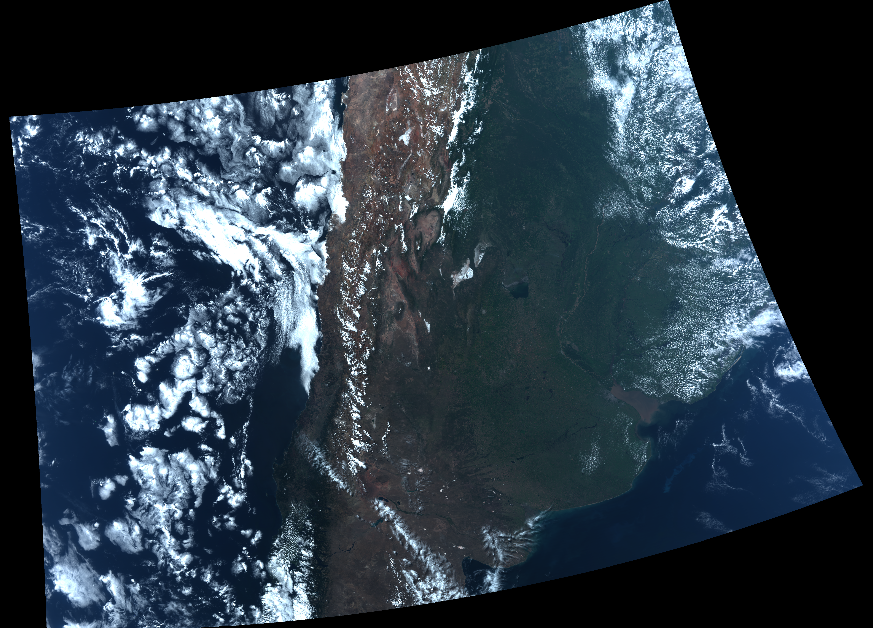
\includegraphics[height=10cm,keepaspectratio=true,clip=true]{imagenes/recoleccion/img-543.png}
  \caption{Combinación de bandas M5, M4 y M3}
	\label{Fig: bandas543}
\end{figure}


%\chapter{Evaluación Experimental}\label{chap:evaluacion}

En este capitulo de expondrá los resultados que se obtuvieron por medio de los experimentos realizados. Los pasos seguidos serán presentados dividiendo en diferentes secciones para lograr una mayor comprensión en el trabajo.

La primera sección \textit{Preparación de Datos} \ref{sec:preparacion_de_datos}, se muestran cuales fueron los datos finales para realizar los experimentos.

La segunda sección  \textit{Entrenamiento y Validación} \ref{sec:entrenamiento}, se detallan como se realizo el proceso de aprendizaje de los datos y los procesos de validación realizados.

\section{Preparación de Datos}\label{sec:preparacion_de_datos}

Vamos a partir de las imágenes obtenidas en el capitulo \ref{chap:recoleccion} donde se puso en detalle los tipos de imágenes que serán utilizadas. En esta sección hablaremos de cual es el \textit{ground truth}, región verdadera, utilizada; como se realizo la extracción de característica de cada imagen, y que criterio de selección de candidatos se utilizo para el entrenamiento.

\subsection{Ground truth}\label{sub:groundtruth}

El problema abordado es un problema de clasificación supervisada, es por esto que debemos saber anticipadamente donde se encuentra el objeto de interés que deseamos detectar. En \ac{ml} el termino \textit{ground truth} hace referencia a la información provenida desde la observación; \textit{ground truth} involucra a un conjunto de imágenes y un conjunto de etiquetas en las imágenes que incluye la locación y las características claves en la imagen.

Las etiquetas se añadieron manualmente utilizando una librería desarrollada en python llamada \textit{labelme}\footnote{Fuente: 
https://github.com/wkentaro/labelme}; que nos permite realizar las anotaciones de las zonas de interés sobre la imagen.

\begin{figure}[h]
 \centering
  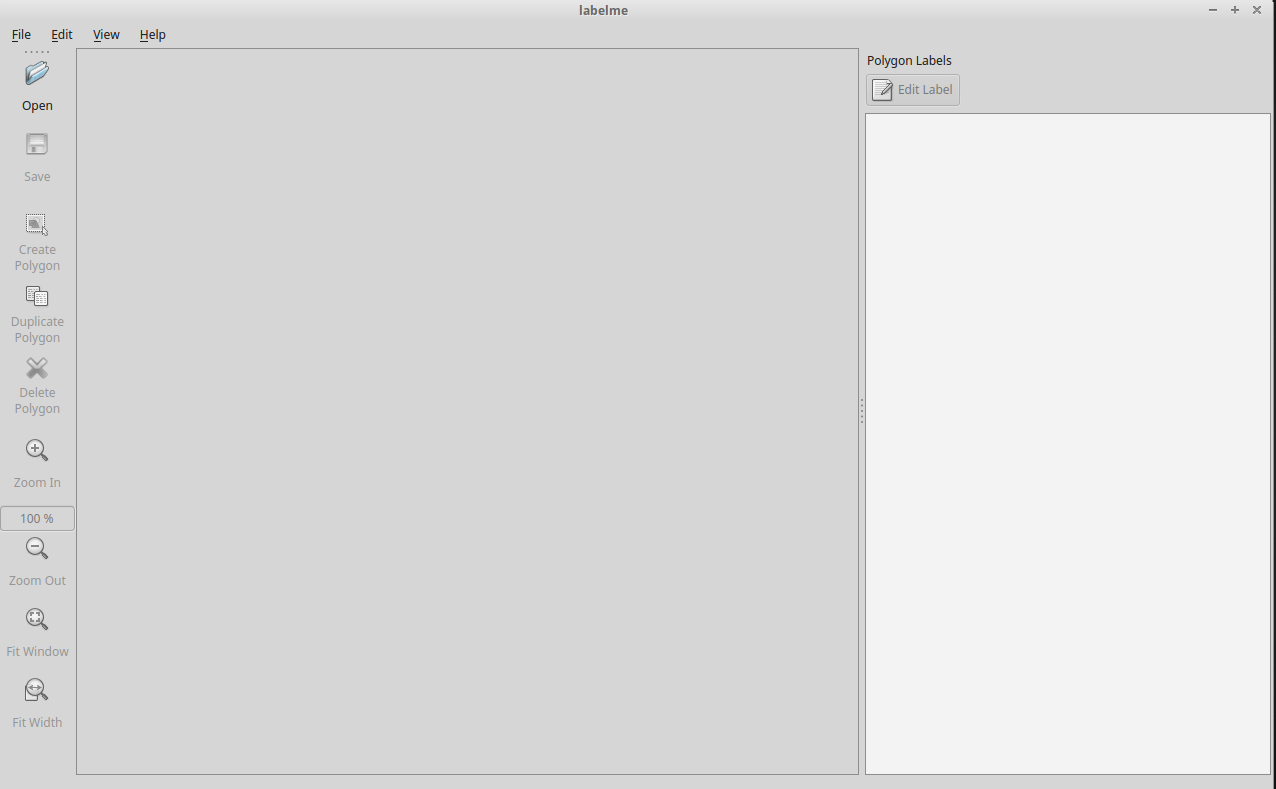
\includegraphics[height=9cm,keepaspectratio=true,clip=true]{imagenes/Logos/labelme.png}
  \caption{Pantalla Principal \textit{labelme}}
	\label{Fig: labelme}
\end{figure}

En las imágenes siguientes se muestra el proceso de anotación que se llevo a cabo mediante \textit{labelme}, para detalles de la instalación ir a: \ref{sec:instalacionlabelme}.

Cada anotación se almacena en un archivo .json que luego es transformado y almacenado en una tabla como vemos en \ref{tab:ejemGT}
\begin{figure}[h]
 \centering
  \includegraphics[height=8cm,keepaspectratio=true,clip=true]{imagenes/Logos/labelme1.png}
  \caption{Etiquetar una región en \textit{labelme}}
	\label{Fig: labelme1}
\end{figure}

\begin{figure}[H]
 \centering
  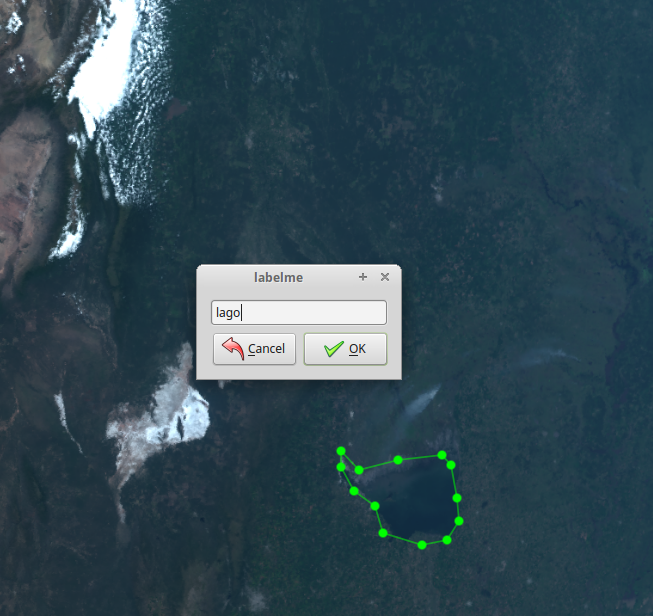
\includegraphics[height=10cm,keepaspectratio=true,clip=true]{imagenes/Logos/labelme2.png}
  \caption{Etiquetar una región en \textit{labelme}}
	\label{Fig: labelme2}
\end{figure}

El \textit{ground truth} final obtenido se guardo en el siguiente formato de anotación (ver \ref{tab:GT} y \ref{tab:ejemGT}):

\begin{table}[H]
\begin{center}
\begin{tabular}{|c|c|c|c|}
\hline Nombre & Bandas & Región & Puntos anotados(x,y)\\ \hline 
\end{tabular}
\end{center} \caption{Estructura ground truth.}\label{tab:GT}
\end{table}

\begin{table}[H]
\begin{center}
\begin{tabular}{|c|c|c|c|}
\hline \textbf{Nombre} & \textbf{Bandas} & \textbf{Región} & \textbf{Puntos anotados(x,y)}\\ \hline 
Imagen01 & 367 & Lago  & 23,50,55,22,223\\ \hline 
Imagen02 & 543 & Lago  & 55,26		\\ \hline 
Imagen03 & 543 & Golfo & 44,300,500,900 \\ \hline 
.......  & ...  & .....& ...............\\ \hline 
\end{tabular}
\end{center} \caption{Ejemplo ground truth.}\label{tab:ejemGT}
\end{table}


\subsection{Regiones Candidatas}\label{sub:proposal}

Cada una de las imágenes obtenidas (ver: \ref{chap:recoleccion}), se aplico técnicas de selección de regiones candidatas para luego ser analizada y clasificada; para esta fase aplicamos métodos de \textit{Regions Proposal} visto en el capitulo \ref{chap:marcoteorico}.

La primera  consideración tomada fue analizar que método de \textit{Regions Proposal} se utilizaría. Se realizaron pruebas con los métodos \ac{bing}, Selective Search y Edge Boxes; donde podemos detallar lo siguiente: \ref{tabla:comparacionregiones}.

\begin{table}[H]
\centering
\begin{tabular}{|p{2cm}|p{6cm}|p{8cm}|}
    \hline 
     & \centering \textbf{Ventajas} & \multicolumn{1}{c|}{\centering \textbf{Desventajas}} \\
    \hline
    \centering Selective Search & \parbox[p][0.2\textwidth][c]{6cm}{
    \begin{itemize}
        \item Fácil implementación en python	
    \end{itemize}}  &  \parbox[p][0.2\textwidth][c]{7.5cm}{
    \begin{itemize}
        \item Tiempo de ejecución muy alto para imágenes de resolución mayores; ejemplo: 2800x3000px.	
    \end{itemize} } \\ \hline
    \centering Edges Boxes & \parbox[p][0.2\textwidth][c]{6cm}{
    \begin{itemize}
        \item Buen tiempo de ejecución con imágenes de gran tamaño
        \item Reconocimientos de regiones de menor tamaño
    \end{itemize} } & \parbox[p][0.2\textwidth][c]{7.5cm}{
    \begin{itemize}
        \item No se encontró una implementación optima en python.	
    \end{itemize} } \\ \hline 
     \centering BING & \parbox[p][0.2\textwidth][c]{6cm}{
    \begin{itemize}
        \item El tiempo de ejecución en imágenes de gran tamaño es optimo
    \end{itemize} } &  \parbox[p][0.2\textwidth][c]{7.5cm}{
    \begin{itemize}
        \item Baja probabilidad de encontrar regiones de menor tamaño en imágenes grandes.
    \end{itemize} } \\ \hline
\end{tabular}
\caption{Análisis de métodos Regiones Propuestas}
\label{tabla:comparacionregiones}
\end{table}

Unos de los principales inconvenientes a la hora del desarrollo de la tesis fue el tamaño de las imágenes. Las regiones de interés son mas pequeñas en proporción a la escala y tamaño de la imagen utilizada, por este motivo al aplicar técnicas de selección de candidatos no generalizaba de manera correcta las regiones que deseamos captar. Para eliminar este problema se procedió a realizar los siguientes pasos: 
\begin{enumerate}
 \item Para cada imagen original se corto en regiones de 256px de alto por el ancho total de la imagen (ver: \ref{Fig: cropimagen}), donde \textit{w} es el ancho de la imagen y \textit{h} alto de la imagen
 \item Se aplico para cada recorte obtenido el método \textit{Edges Boxes} para la obtención de regiones candidatas (ver: \ref{Fig: cropproposal}).

\begin{figure}[H]
 \centering
  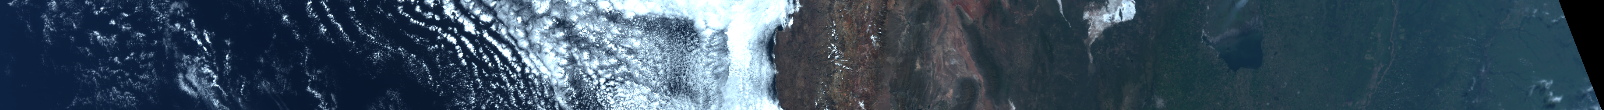
\includegraphics[height=1.2cm,keepaspectratio=true,clip=true]{imagenes/Logos/cropimagen.png}
  \caption{Crop de Imagen Satelital (4833\textit{w} X 256\textit{h})}
	\label{Fig: cropimagen}
\end{figure}

\begin{figure}[H]
 \centering
  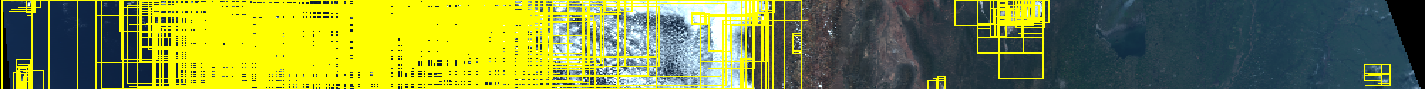
\includegraphics[height=1.1cm,keepaspectratio=true,clip=true]{imagenes/Logos/cropproposal.png}
  \caption{Aplicación de Edges Boxes a un recorte de la imagen.}
	\label{Fig: cropproposal}
\end{figure}

\item Para cada imagen se obtuvo 26 recortes en total, obteniendo el siguiente resultado en la imagen completa \ref{Fig: proposal}.

\begin{figure}[H]
 \centering
  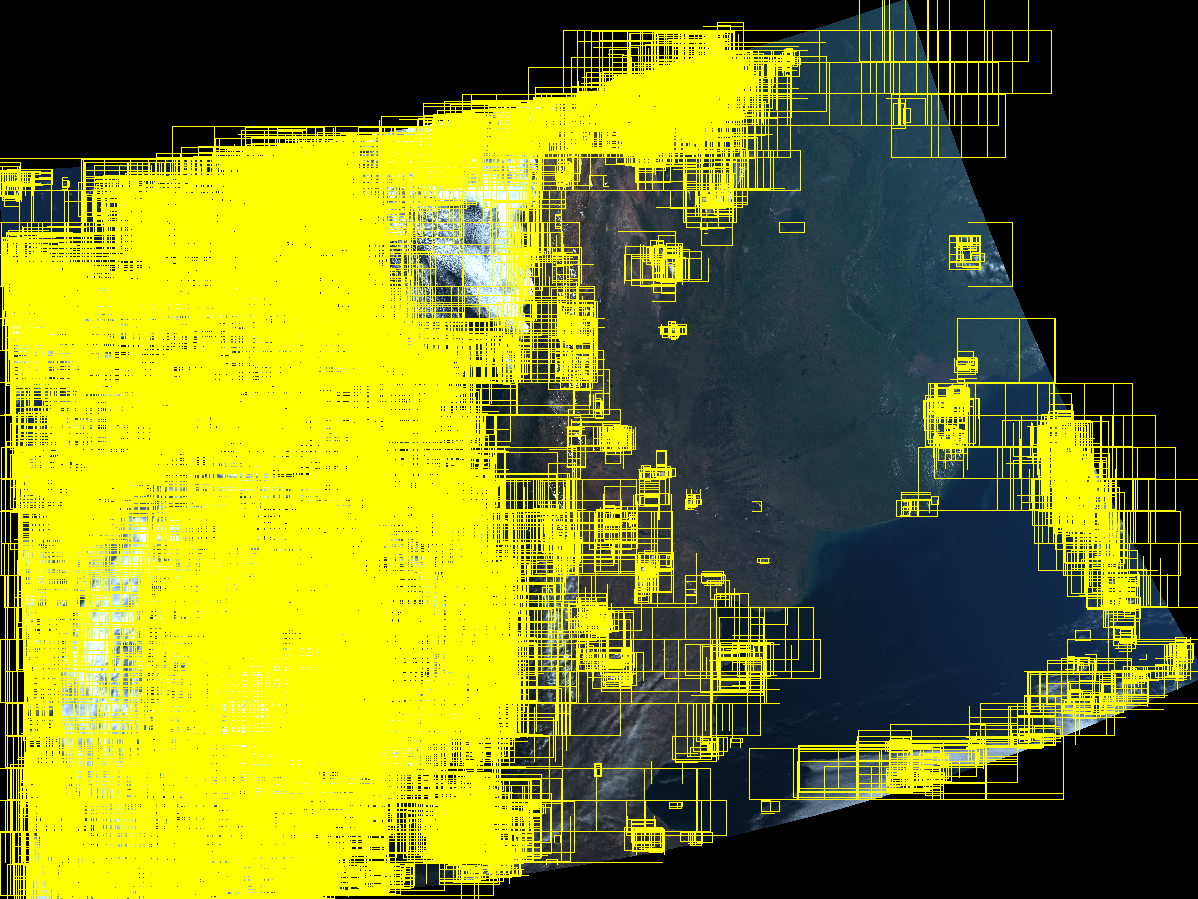
\includegraphics[height=13cm,keepaspectratio=true,clip=true]{imagenes/Logos/proposal.png}
  \caption{Aplicación de Regiones propuestas a una imagen satelital.}
	\label{Fig: proposal}
\end{figure}

\end{enumerate}
La imagen anterior \ref{Fig: proposal} se obtuvo 53.815 regiones por el método \textit{Edges Boxes} de selección de candidatos. Procesar estas 53.815 regiones candidatas consumirá mucho tiempo de computo, además podemos visualizar que existen regiones solapadas (overlapping); estas regiones representan información duplicada que debemos eliminar. 

Para solucionar el problema del \textit{overlapping}  aplicamos \ac{nms} visto en la sección \ref{sec:nonmaximumsuppression}. 
El valor usado para la eliminación de regiones candidatas duplicadas fue de 0.8 como valor de solapamiento entre regiones candidatas detectadas.

En la figura siguiente \ref{Fig: proposalnms} se pude observar que con un valor 0.8 de \textit{overlapping} aplicando \ac{nms} obtenemos un 90\% aproximadamente de optimización en la eliminación de regiones candidatas duplicada, es decir se paso de 53.815 a 1.560 regiones candidatas por imagen para el entrenamiento.

\begin{figure}[H]
 \centering
  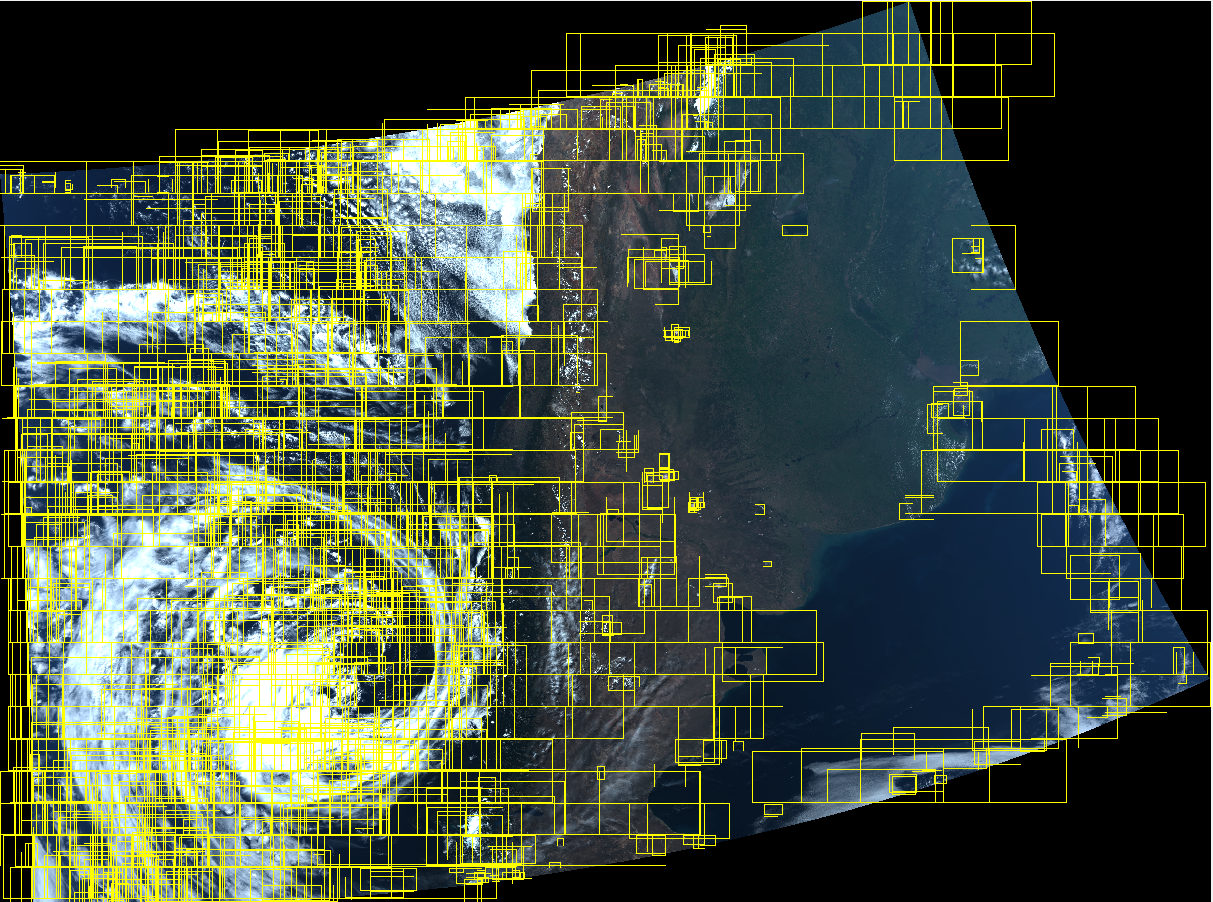
\includegraphics[height=13cm,keepaspectratio=true,clip=true]{imagenes/Logos/proposalconNMS.png}
  \caption{Proposal obtenido con Non-maximum suppression}
	\label{Fig: proposalnms}
\end{figure}


\subsection{Etiquetado}\label{sub:etiquetado}

Los datos obtenidos de la recolección de regiones candidatas a partir de los métodos \textit{Proposal} debe ser etiquetados para su entrenamiento. Para realizar el etiquetado se utilizo el \textit{ground truth} \ref{sub:groundtruth} que serán comparados con las regiones candidatas calculando el \textit{overlapping} entre estas.

El criterio utilizado en el etiquetado de datos es el siguiente:
\begin{enumerate}
	\item 0: NO contiene el patrón de interés en la región candidata.
	\item 1: Existencia del patrón en la región candidata.
\end{enumerate}

Para la selección de alguna de las etiquetas anteriores el umbral de decisión fue de 0.5 como valor de \textit{overlapping}, es decir el nivel de solapamiento que existen entre el \textit{ground truth} y la región candidata.


\subsection{Extracción de Características}\label{sub:extracciondecaracteristica}

El proceso de extracción de característica se realiza sobre la regiones candidatas obtenidas luego de aplicar \ac{nms} sobre estas. Por cada región se obtendrá un vector de 2048 dimensiones que representa las características de esa región encontrada.

La obtención del vector de característica se realiza por medio de una \ac{cnn}, en donde las entradas a la red son las regiones candidatas. Para este proceso se utilizó una red pre-entrenada \textbf{ResNet50} donde se obtuvo de la ante ultima capa el vector que va a representar la región.

Los vectores obtenidos se almacenaron en un archivo de extensión \textit{.mat}; que contiene los siguientes datos:
\begin{itemize}
 \item Las coordenadas de cada regiones candidatas.
 \item El \textit{feature vector} de 2048 elementos que corresponde a cada región. 
 \item Las etiquetas que indica a que clase pertenece la región \ref{sub:etiquetado}.
\end{itemize}



%%%%% PONER EJEMPLO DE CODIGO???? y crop de las alguno de los regions proposal???


\section{Entrenamiento y Validación}\label{sec:entrenamiento}

En esta sección se comparte como se realizo el proceso de aprendizaje automático \ac{ml} con los datos obtenidos de la sección anterior \ref{sec:preparacion_de_datos}. El conjunto de imágenes finales utilizado para el entrenamiento se detalla en \ref{sec:datosutilizados}.

El datasets final se dividió en tres conjuntos:
\begin{itemize}
\item Train.
\item Test.
\item Validation.
\end{itemize}

El total de la muestra de datos para la experimentación fue de 650.000 \textit{feature vector}.

\subsection{Hiper-parametros}\label{sub:hiperparametro}


Para obtener una predicción correcta se debe realizar la optimización de parámetros que afectan a la clasificación. El método utilizado para poder realizar la optimización de estos parámetros fue \textit{grid search}\footnote{Fuente: https://goo.gl/koWr74}.  Grid search busca por fuerza bruta los parámetros a optimizar quedándose con aquel que logre un mayor \textit{accuracy} en las evaluaciones; en cada iteración se utiliza \textit{cross-validation} con 5 folds en el entrenamiento para evitar el \textit{overfitting}.

Los parametros son:
\begin{enumerate}
	\item \textbf{Parámetro C}: Controla el costo de la mala clasificación, \textit{misclassification}, en los datos de entrenamiento. Con un valor de C pequeño hará que el optimizador busque un hiperplano de separación de mayor margen, incluso si ese hiperplano clasifica erróneamente más puntos. Para valores muy pequeños de C, debe obtener ejemplos mal clasificados, a menudo incluso si sus datos de entrenamiento son linealmente separables. Para valores grandes de C,  elegirá un hiperplano de menor margen si ese hiperplano hace un mejor trabajo de conseguir que todos los puntos de entrenamiento estén clasificados correctamente. El objetivo es encontrar el equilibrio entre "no demasiado estricto" y "no demasiado relajado". La validación cruzada  son buenas maneras de encontrar el mejor C.
	\item \textbf{Parámetro gamma}: Es la inversa de la desviación estándar del kernel RBF (función gaussiana), que se utiliza como medida de similitud entre dos puntos.
\end{enumerate}
	

El rango de parámetros usados para el entrenamiento y validación de datos fueron los siguientes:

\begin{itemize}
 \item \textbf{Valor de C}: 1000,100,10,1, 0.1,0.01,0.001,0.0001
 \item \textbf{Valor de Gamma}: 1,0,1,0,01,0,001,0,0001,0,00001
\end{itemize}




\subsection{Metricas}\label{sub:metricas}

Además de la optimización de los parámetros mencionados \ref{sub:hiperparametro}, la validación de los resultados se usaron las siguientes métricas: \textit{Accuracy, Precisión y Recall}.

\begin{itemize}
	\item Positivos (P): Observación positiva (valor etiquetado).
	\item Verdadero Positivo (TP): La observación es positiva y la predicción también.
	\item Falso Negativo (FN): La observación es positiva pero la predicción es negativa.
	\item Falso Positivo (FP): La observación es negativa pero la predicción es positiva.
	\item Verdadero Negativo (TN) :  La observación es negativa y también la predicción negativa.
\end{itemize}

\begin{enumerate}
\item \textbf{Accuracy:} Proporción de todas las predicciones que son correctas; da una medida de que tan bueno es el modelo.
\begin{equation}
accuracy = \frac{FP+FN}{FP+FN+TP+TN}=\frac{predicciones\;correctas}{todas\;las\;predicciones}
\end{equation}

\item \textbf{Precisión:} Proporción de todas las predicciones positivas que son correctas. La precisión es una medida de cuántas predicciones positivas son reales.
\begin{equation}
precision=\frac{TP}{TP+FP}= \frac{predicciones\;correctamente\;positivas}{todas\;las\;predicciones\;positivas}
\end{equation}

\item \textbf{Recall:} Nos da la proporción de la observaciones reales positivas que son correcta, es decir nos da la precisión de cuantas observaciones positivas reales se obtuvo correctamente.
\begin{equation}
recall = \frac{TP}{TP+FN} = \frac{TP}{P} = \frac{predicciones\;a\;ser\;positiva}{todas\;la\;observaciones\;positivas} 
\end{equation}

\item \textbf{Overlapping Mean:} Métrica obtenida a partir de la intersección del ground truth y el bounding box de la predicción obtenida.

\end{enumerate}


\subsection{Resultados obtenidos}\label{sub:resultados}

En la siguiente tabla \ref{tab:entrenam-result}	se expone los resultados obtenidos de los entrenamientos realizados. Como podemos ver se consideraron  diferentes combinaciones de banda con el fin de encontrar aquella que mejoren las métricas y que resalten las zonas de interés que deseamos detectar.

\begin{table}[H]
\begin{center}
\begin{tabular}{|c|c|c|c|c|c|c|c|}
\hline
 & \multicolumn{3}{c|}{Hiper - parametros} & \multicolumn{4}{c|}{Metricas} \\ \hline
Bandas & C & gamma & kernel & precision & recall & \begin{tabular}[c]{@{}c@{}}average\\ presicion\end{tabular} & \begin{tabular}[c]{@{}c@{}}overlapping\\ mean\end{tabular} \\ \hline
\multicolumn{1}{|c|}{1-1-1} & 10 & - & linear & 0.91 & 0.91 & 0.18 & 0.1 \\ \hline
\multicolumn{1}{|c|}{1-3-5} & 10 & - & linear & 0.93 & 0.94 & 0.57 & 0.28 \\ \hline
\multicolumn{1}{|c|}{1-5-3} & 1000 & 0.01 & rbf & 0.94 & 0.94 & 0.61 & 0.27 \\ \hline
\multicolumn{1}{|c|}{3-1-5} & 100 & 0.01 & rbf & 0.93 & 0.94 & 0.61 & 0.31 \\ \hline
\multicolumn{1}{|c|}{3-3-3} & 1000 & 1 & rbf & 0.92 & 0.92 & 0.28 & 0.1 \\ \hline
\multicolumn{1}{|c|}{3-5-1} & 10 & 0.01 & rbf & 0.90 & 0.91 & 0.66 & 0.25 \\ \hline
\multicolumn{1}{|c|}{5-1-3} & 1 & 1 & rbf & 0.89 & 0.86 & 0.46 & 0.29 \\ \hline
\multicolumn{1}{|c|}{5-3-1} & 1000 & 0.001 & rbf & 0.90 & 0.88 & 0.38 & 0.21 \\ \hline
\multicolumn{1}{|c|}{5-5-5} & 100 & 0.01 & rbf & 0.89 & 0.85 & 0.63 & 0.26 \\ \hline
\multicolumn{1}{|c|}{7-7-7} & 1000 & 0.001 & rbf & 0.92 & 0.92 & 0.75 & 0.30 \\ \hline
\multicolumn{1}{|c|}{9-9-9} & 10 & 1 & rbf & 0.82 & 0.75 & 0.34 & 0.1 \\ \hline
\multicolumn{1}{|c|}{11-7-9} & 1000 & 0.001 & rbf & 0.91 & 0.86 & 0.59 & 0.24 \\ \hline
\multicolumn{1}{|c|}{11-9-7} & 10 & - & linear & 0.91 & 0.89 & 0.74 & 0.26 \\ \hline
\multicolumn{1}{|c|}{7-11-9} & 1 & 1 & rbf & 0.91 & 0.87 & 0.60 & 0.27 \\ \hline
\multicolumn{1}{|c|}{7-9-11} & 10 & - & linear & 0.90 & 0.89 & 0.73 & 0.28 \\ \hline
\multicolumn{1}{|c|}{9-11-7} & 1 & 1 & rbf & 0.89 & 0.86 & 0.66 & 0.23 \\ \hline
\multicolumn{1}{|c|}{9-7-11} & 1 & 1 & rbf & 0.89 & 0.86 & 0.79 & 0.30 \\ \hline
\multicolumn{1}{|c|}{11-11-11} & 1 & 1 & rbf & 0.91 & 0.88 & 0.74 & 0.27 \\ \hline
\multicolumn{1}{|c|}{11-3-15} & 10 & 0.1 & rbf & 0.89 & 0.83 & 0.59 & 0.3 \\ \hline
\multicolumn{1}{|c|}{11-15-13} & 1 & 1 & rbf & 0.89 & 0.84 & 0.63 & 0.28 \\ \hline
\multicolumn{1}{|c|}{13-11-15} & 10 & - & linear & 0.89 & 0.87 & 0.61 & 0.26 \\ \hline
\multicolumn{1}{|c|}{13-13-13} & 1 & - & linear & 0.91 & 0.90 & 0.32 & 0.35 \\ \hline
\multicolumn{1}{|c|}{13-15-11} & 1 & - & linear & 0.89 & 0.82 & 0.39 & 0.26 \\ \hline
\multicolumn{1}{|c|}{15-11-13} & 10 & 1 & rbf & 0.89 & 0.86 & 0.51 & 0.25 \\ \hline
\multicolumn{1}{|c|}{15-13-11} & 1000 & 0.001 & rbf & 0.90 & 0.86 & 0.54 & 0.27 \\ \hline
\multicolumn{1}{|c|}{15-15-15} & 10 & 1 & rbf & 0.88 & 0.85 & 0.26 & 0.28 \\ \hline
\multicolumn{1}{|c|}{11-12-13} & 1000 & 1 & rbf & 0.87 & 0.91 & 0.62 & 0.32 \\ \hline
\multicolumn{1}{|c|}{5-4-3} & 1000 & 1 & rbf & 0.88 & 0.87 & 0.57 & 0.27 \\ \hline
\multicolumn{1}{|c|}{10-7-5} & 1000 & 0.001 & rbf & 0.91 & 0.96 & 0.58 & 0.36 \\ \hline
\end{tabular}
\end{center}\caption{Resultados de los entrenamientos}\label{tab:entrenam-result}
\end{table}

Cada uno de los valores encontrados de los hiper parámetros se obtuvo a través de \textit{grid search}, estos valores son los que optimizan las métricas que estamos empleando.

Se evaluaron también las detecciones obtenidas en el conjunto de test evaluando los \textit{falsos positivos} y re entrenando nuevamente el clasificador con los falsos positivos obtenidos con el fin de lograr una mejora en la detección y localización de las regiones que estamos buscando.

Las tareas realizadas para evaluar la localización del objeto fue obtener el \textit{overlapping mean}; en esta métrica comparamos los \textit{bounding boxs} obtenidos en el entrenamiento realizado y el \textit{ground thruth}, región de interés, que tenemos anotado. Este valor nos da una visión de cual es la exactitud de nuestro predictor en cuanto a la localización del objeto.

En el siguiente cuadro se visualiza la relación existente entre las regiones detectado y la presicion de la detección \ref{Fig: trade-off}.


\begin{figure}[H]
 \centering
  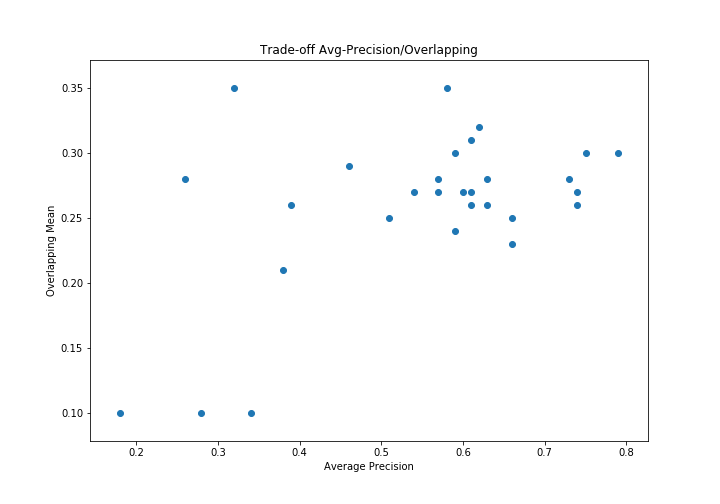
\includegraphics[height=9cm,keepaspectratio=true,clip=true]{imagenes/Evaluacion-exp/presicion-over.png}
  \caption{Trade-Off Average Presicion-Overlapping}
	\label{Fig: trade-off}
\end{figure}

La siguiente imagen se puede visualizar los \textit{bounding boxs} detectados, esto es el resultado de aplicar el modelo entrenado a una imagen satelital; en este caso la imagen utilizada pertenece a las bandas M9-M7-M11, como se puede ver en la tabla \ref{tab:entrenam-result}, esta combinación de banda es una de las que mejores metricas se obtuvo en terminos de localización y presicion en los entrenamientos.


\begin{figure}[H]
 \centering
  \includegraphics[height=9cm,keepaspectratio=true,clip=true]{imagenes/Evaluacion-exp/prediction-9711.png}
  \caption{Ejemplo de predicciones positivas}
	\label{Fig: TP}
\end{figure}

%\chapter{Conclusiones y lineamientos futuros}\label{chap:conclusiones}


\section{Conclusiones}
En el desarrollo de la presente tesis se abordo un problema de detección buscando patrones de interés, laguna Mar Chiquita y golfo de San Matías, dentro de una imagen satelital. Para la construcción de la solución se utilizaron diferentes técnicas para el pre-procesamiento de la imagen, redes neuronales para la extracción de característica y algoritmos de clasificación. 

Como resultado de todos los experimentos realizados se puede exponer las siguientes conclusiones:

\begin{enumerate}
\item Utilizar técnicas de aprendizaje automático en el proceso de automatización de tareas, como en este caso la detección de patrones en una imagen satelital, nos brinda una fuente de información extra para poder realizar el proceso de calibración/detección que se busca en el satélite. 

\item Al trabajar con imágenes satelitales en donde las resoluciones de la misma son grandes, se debe tener en cuenta el tamaño de la regiones de interés que se quiere detectar.

\item Uno de los puntos importantes es el tipo del hardware que vamos a utilizar, el cómputo de los vectores de característica utilizando redes neuronales es costoso en términos de memoria y velocidad, es por este motivo que en la mayoría de los casos de uso utilizan GPU para el procesamiento.

\item En base a las experimentaciones realizadas podemos afirmar que aplicar redes neuronales pre-entrenadas para la extracción de característica se obtiene una correcta generalización de los datos y son muy eficiente para problemas de clasificación de imágenes.

\item Unos de los principales inconvenientes detectados fue el \textit{overfitting} de los datos, esto se debió al desbalanceo de clases ya que se recolectó muy pocas muestras positivas, en la mayoría de los casos debido a las nubes que interceptaban la región de interés buscada. Se soluciono este problema usando técnicas de cross-validation.

\end{enumerate}

El costo computacional en término de capacidad de operaciones hace que utilizar técnicas de \ac{cv} sea  muy costoso de aplicar en vuelo. Unos de los principales inconvenientes son la limitaciones de energía que posee un micro-nano-satélite, es por esto que se torna inviable en términos de energía y capacidad de almacenamiento poder implementar esta tecnología. No obstante pudimos ver que herramientas como \ac{ml} y \ac{cv} ayudan de manera eficiente a detectar elemento sobre una imagen satelital automatizando los procesos.



\section{Lineamientos futuros}\label{lineafuturas}
Tomando como base las lecciones aprendidas en el desarrollo de la tesis, las posibles lineas de trabajo e investigaciones a futuro son:
\begin{enumerate}
 \item A partir del bajo rendimiento en el cálculo de los datos surge la posibilidad de implementar procesamiento en base a GPU para el cómputo en paralelo de los las imágenes.
 \item Es posible aplicar diferentes arquitectura de las redes neuronales para la extracción de los vectores de característica; de esta manera determinar cual de las redes tiene mayor generalización en los datos para el tipo de problemática que estamos tratando.
 \item Evaluar nuevas herramientas de extracción de características y computar redes mucho más livianas en términos de consumo de energía.
\end{enumerate}

\bibliografia{template_tesis_mdiae.bib}
%\bibliographystyle{apalike}
\bibliographystyle{apa}
%\bibliography{#1}
%\nocite{*}
%------------------------------------------------------------------------------
% EN CASO DE TENER APÉNDICES, DESCOMENTAR A CONTINUACIÓN
\appendix
\chapter{ANEXO}\label{chap:anexo}
%\section{Instalación Labelme}\label{sec:instalacionlabelme}
%La instalación de \textit{labelme}, se realizo bajo un sistema operativo Ubuntu-Linux Mint v18.0; se debe instalar las siguiente dependencias:
%\href{https://www.scipy.org/}{Scipy},\href{http://www.numpy.org/}{Numpy},\href{http://scikit-image.org/}{scikit-image}
%,\href{https://riverbankcomputing.com/software/pyqt/intro}{PyQt}, \href{http://matplotlib.org/}{Matplot}


%Luego desde la terminal de Linux ingresamos los siguientes comandos:

%\textbf{(user):sudo apt-get install labelme}

%Para iniciar \textit{labelme} se ingresa desde la terminal el siguiente comando:

%\textbf{(user): labelme (path/nameimage.tiff)}

%\begin{figure}[H]
% \centering
%  \includegraphics[scale=0.3,keepaspectratio=true,clip=true]{imagenes/Apendice/labelme1.png}
%  \caption{Pantalla Principal \textit{labelme}}
%	\label{Fig: labelme}
%\end{figure}

%Las anotaciones realizas en este software se almacenará en formato JSON.

%%%%%%%%%%%%%%%%%%%%%%%%%%%%%%%%
%\section{Instalación Keras}\label{sec:instalacionkeras}
%Keras es una librería para hacer Deep Learning, keras esta escrita en python ejecuntandose sobre una capa superior de TensorFlow. A continuación vamos a desarrollar el proceso de instalación:

%Dependencias de Keras:
%\begin{itemize}
%\item numpy scipy
%\item scikit-learn
%\item pillow
%\item h5py
%\end{itemize}
%Luego de la instalación de las dependencias hacemos:

 %\textbf{\$ sudo pip install keras}
%%%%%%%%%%%%%%%%%%%%%%%%%%%%%%%%
%\section{Instalación OpenCV}\label{sec:instalacionopencv}
%La instalación de OpenCV se realizo por medio del Repositorio de Ubuntu:

%\$\textbf{ sudo pip install opencv-python}

%La versión utilizada de OpenCV fue la 2.4.9.1 bajo Ubuntu 14.04. Para verificar la su instalación realizamos los siguiente:\\
%\$ python\\
%\$ import cv2\\
%\$ cv2.\_version\_


%%%%%%%%%%%%%%%%%%%%%%%%%%%%%%%%


%%%%%%%%%%%%%%%%%%%%%%%%%%
\section*{Descargas y Recolección de Imágenes}\label{sec:descargas_img}
Se descargaron las imágenes del sitio de la pagina oficial de \ac{conae} \url{http://www.conae.gov.ar/index.php/espanol/}, para la obtención de las imágenes nos dirigimos a
la solapa \textit{Catálogo de imágenes y productos}:

\begin{figure}[H]
 \centering
  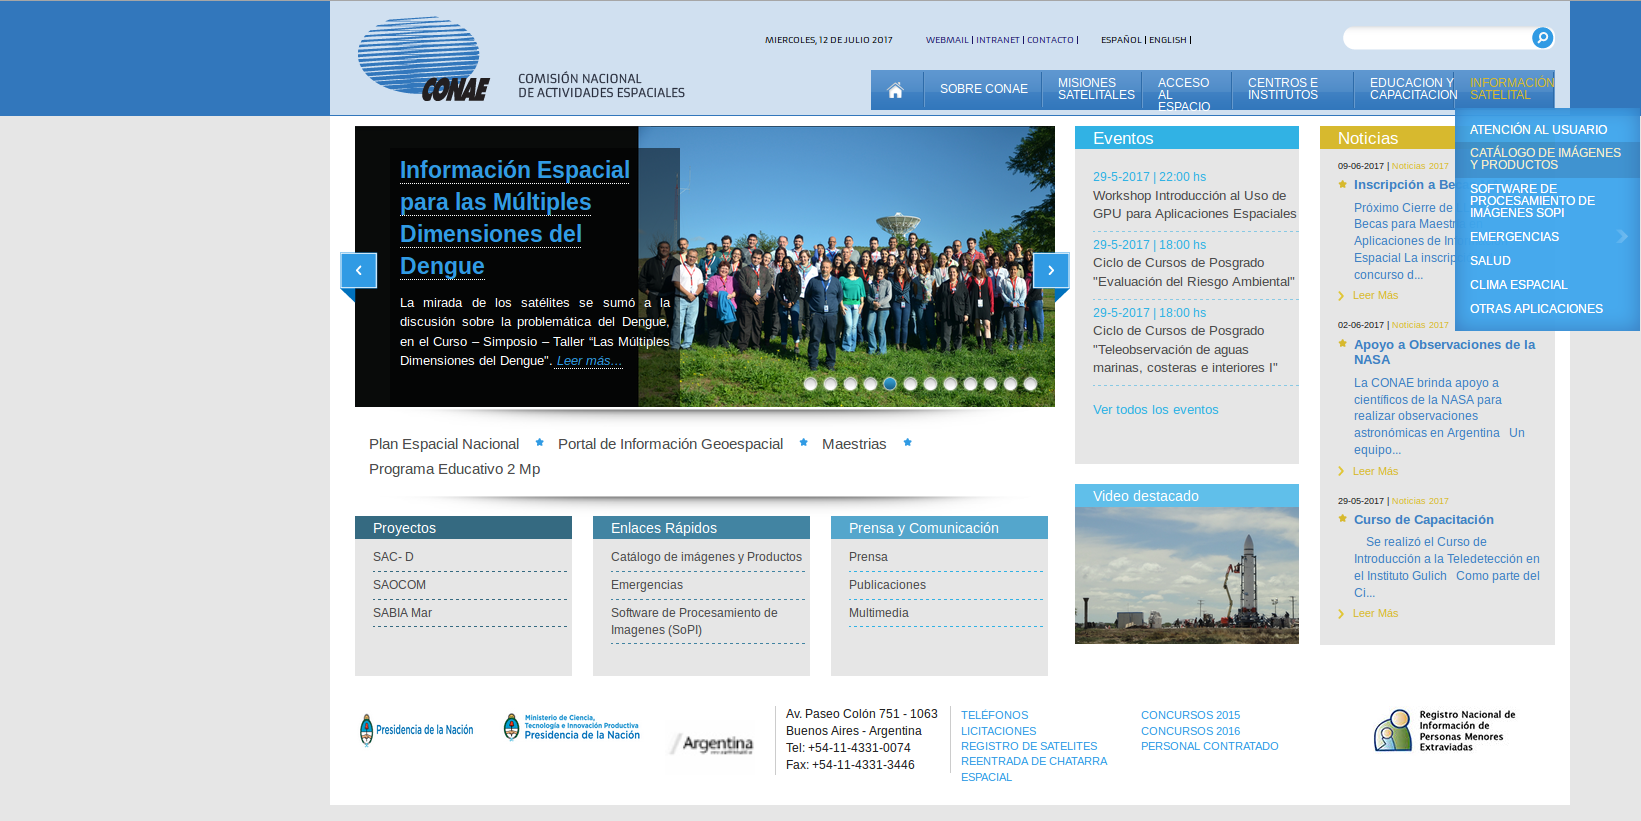
\includegraphics[scale=0.2,keepaspectratio=true,clip=true]{imagenes/Apendice/conaepag.png}
  \caption{Pantalla Principal CONAE}
\end{figure}

Luego en las secciones de la izquierda de la pagina seleccionamos Aqua, Terra correspondiente al sensor modis o NPP para viirs.
\begin{figure}[h]
 \centering
  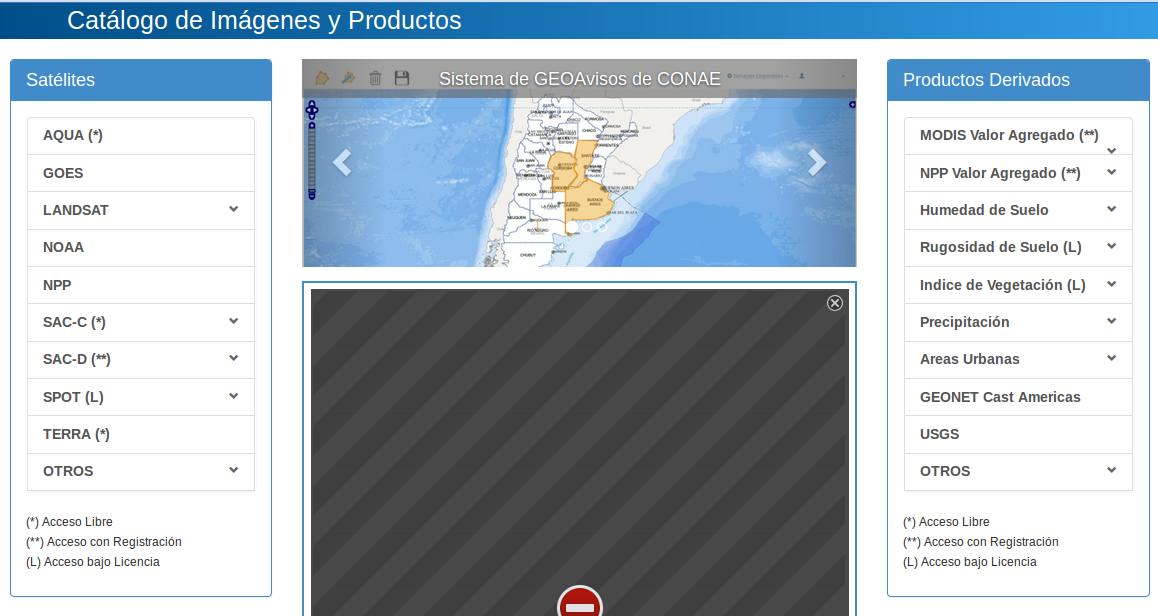
\includegraphics[scale=0.3,keepaspectratio=true,clip=true]{imagenes/Apendice/conaepag1.png}
  \caption{Pantalla Principal CONAE}
\end{figure}
Para la descargas de las imágenes se debe autenticar, si no posee un usuario debe darse de alta en el sistema. Una vez autenticado podemos buscar por fecha, región, latitud,
longitud o nombre de la imagen.
\begin{figure}[h]
 \centering
  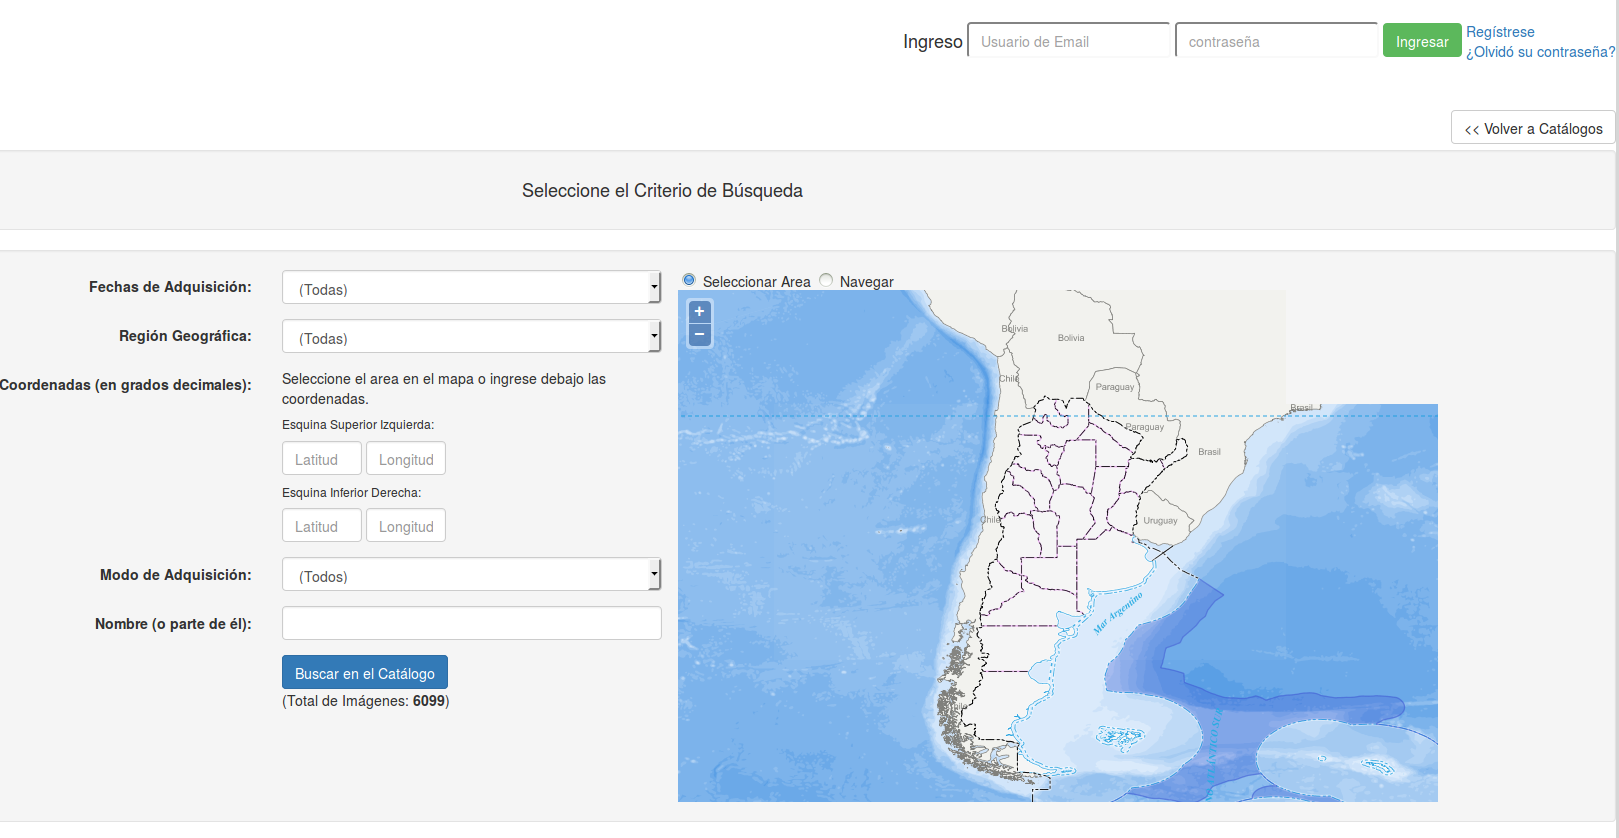
\includegraphics[scale=0.2,keepaspectratio=true,clip=true]{imagenes/Apendice/conaepag2.png}
  \caption{Autenticación de usuario}
\end{figure}
Una vez seleccionada la imagen a descargar nos aparece las características de la imagen junto con las bandas que deseamos y su correspondiente archivo de georeferenciación.
\begin{figure}[H]
 \centering
  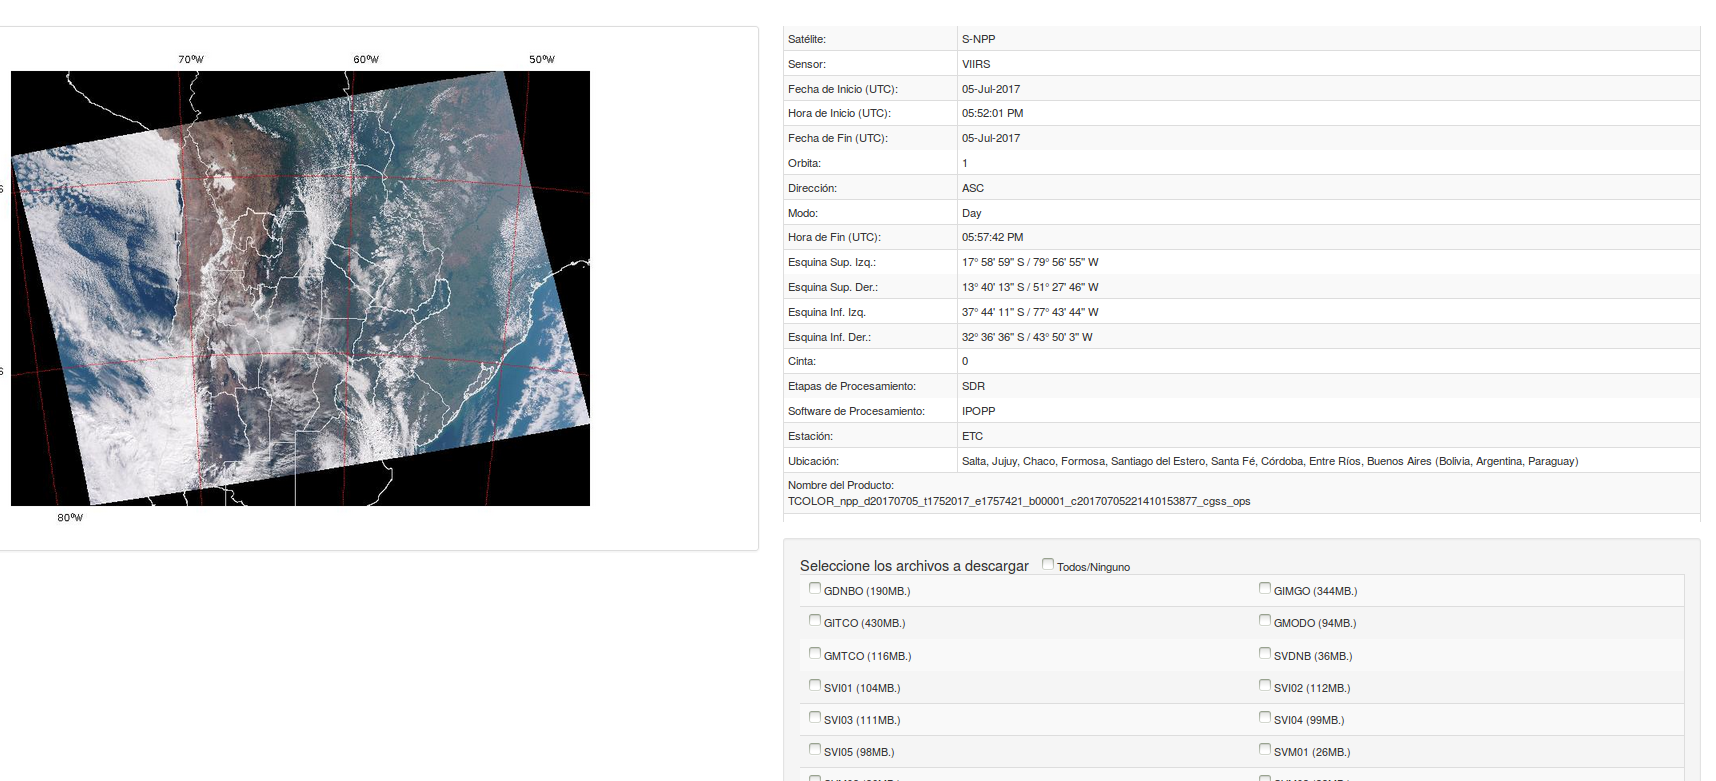
\includegraphics[scale=0.2,keepaspectratio=true,clip=true]{imagenes/Apendice/conaepag3.png}
  \caption{Descarga de Imagen}
\end{figure}

\section*{Desarrollo del Software}\label{sec:Desarrollo}

El capitulo siguiente se describirá las diferentes herramientas de software utilizadas para el desarrollo de esta tesis. El mismo se dividirá en dos secciones la primera describe los detalles técnicos como lenguaje de programación, librerías de software y entorno de trabajo; la segunda sección se muestra la organización y estructura del código realizado.


\subsection*{Detalles Técnicos e Implementación}\label{sec:implementacion}

\subsubsection*{Python}
Python es un lenguaje de programación de código abierto y multiparadigma que permite la programación orientada a objeto, funcional e imperativa. 
Cuenta con estructuras de datos eficientes y de alto nivel, el interprete de Python puede extenderse fácilmente  con nuevas funcionalidades y tipos 
de  datos implementados en C o C++, además cuenta con una amplia comunidad de soporte y 
documentación \footnote{Fuente:www.docs.python.org.ar/tutorial}. 

Los principales motivos por el cual se optó por este lenguaje de programación es:
\begin{itemize}
 \item Facilidad de implementación y manipulación de grandes cantidades de datos.
 \item Lenguaje muy utilizado en el ámbito laboral de \ac{ml}.
 \item Posee diversas librerías para \ac{ml} y \ac{cv} en manipulación de datos e imágenes.
\end{itemize}


\subsubsection*{OpenCV}
\ac{opencv}, es una librería de código libre que nos permite manipular imágenes de manera mas eficiente; esta librería se usa en diferentes ámbitos no solo académico, sino también en ámbitos comerciales, como ejemplo en sistemas de seguridad para detección de movimiento, control de procesos, control de calidad de alimentos, automatización de vehículos y en numerosas áreas de la ciencia como robótica, detección de objetos, reconstrucciones 3D, realidad aumentada, etc. \footnote{Fuente: http://opencv.org/} La biblioteca \ac{opencv} puede ser usado bajo licencia BSD (Berkeley Software Distribution) \footnote{Fuente: https://blog.desdelinux.net/hablemos-de-la-licencia-bsd/ } para proyectos escolares o comerciales. 

\subsubsection*{Keras}

Es una interfaz de programación (API) de alto nivel para redes neuronales, escrita en python , para la manipulación y uso de modelos de \ac{cnn}. Envuelve las eficientes bibliotecas de cálculo numérico Theano y TensorFlow y permite definir y entrenar modelos de redes neuronales en unas breves líneas de código \footnote{Fuente:  https://keras.io/}. Como principal inconveniente encontrado es la escasa documentación de la librería.

\subsubsection*{Scikit-Learn}\label{sub:sklearn}
Scikit-Learn es una librería de software desarrollada en Python para solucionar problemas de \ac{ml}; que comprende en intentar predecir datos desconocidos a partir de modelos creados. Cuenta con varios algoritmos para la solución de problemas de ,regresión, clasificación y clustering, incluyendo algoritmos como maquinas de soporte vectoriales, vecino mas cercano (K-NN), descenso de gradiente , entre otros\footnote{Fuente: http://scikit-learn.org/stable/index.html}.

Su principal ventaja es la fácil implementación y manipulación de los algoritmos contenidos en la librería.

\subsubsection*{Entorno de desarrollo}
El entorno de desarrollo utilizado fue el ID \textit{Eclipse}, herramienta de código abierto multiplataforma. Esta herramienta fue diseñada para ser extendida de forma indefinida a través de \textit{plug-ins}. Sus principales características son:
\begin{itemize}
 \item Perspectivas, editores y vistas
 \item Gestión de proyectos
 \item Extensa colección de \textit{plug-ins}
\end{itemize}
El \textit{plug-ins} utilizado para el desarrollo de la tesis fue \textit{Pydev, EGit}. El principal inconveniente encontrado de esta herramienta es 
el consumo de memoria en ejecución, así también se presentaron inconvenientes a la hora de realizar integración en entornos colaborativos como Git.

\subsubsection*{Control de Versiones}

Las herramientas que se utilizaron para llevar un control del versiones en el desarrollo fueron: \textit{GitHub}\footnote{Fuente: https://github.com/} y \textit{GitLab} \footnote{Fuente : https://about.gitlab.com/} , son software pensado en el mantenimiento de aplicaciones. El objetivo de estas aplicaciones gestionar los diversos cambios que se realizaron sobre los elementos de algún producto o alguna configuración del mismo; una versión, revisión o edición del producto, es el estado en el cual se encuentra el mismo.

Las características principales son: herramientas gráficas para ver como se trabajo en el proyecto, entorno colaborativo permitiendo a diferentes desarrolladores compartir sus trabajos, registro histórico de cada acción realizada en cada elemento, seguimiento de errores.

\section*{Organización y Estructura del código}\label{sec:estructuracodigo}

La organización del código experimental se dispuso en varios componentes separados con el fin de hacer el código mas re-utilizable.

La estructura del directorio de trabajo es la siguiente:
\begin{itemize}
 \item \textbf{CNN}: Las funciones que contiene realizan el calculo del \textit{feature vector} a través de una red neuronal utilizando la librería 
\textit{Keras}.
 \item \textbf{ImgManipulation}: Almacena las diferentes funciones que permiten la manipulación de las imágenes de entrada 
 \item \textbf{Notacion}: Contiene diferentes clases que permiten calcular los bounding box y \ac{nms}; también contiene las funciones que almacenan 
la notaciones.
 \item \textbf{Proposal}: Contiene la clase que ejecuta regions proposal.
 \item \textbf{TensorF}:Almacena las funciones que permiten realizar el entrenamiento de los datos utilizando \textit{Scikit-Learn}.
\end{itemize}

\begin{figure}[H]
 \centering
  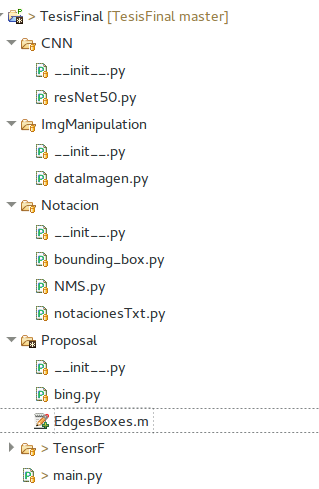
\includegraphics[scale=0.4,keepaspectratio=true,clip=true]{imagenes/Logos/structureData.png}
  \caption{Estructura de directorio de trabajo}
\end{figure}


\textbf{main.py}\\
Este scripts constituye la parte principal del proceso automatizado; llamando a las diferentes clases mencionadas previamente. Las principales 
acciones que lleva a cabo son:
\begin{itemize}
 \item Lee las carpetas que contiene las imágenes junto con las anotaciones de cada una de ellas.
 \item Comprueba que exista las notaciones
 \item A cada imagen realiza el crop(recorte) correspondiente.
 \item Extrae las anotaciones de cada imagen.
 \item Llama a la clase para calcular \textit{regions proposal}.
 \item Calcula el \textit{overlapping}, \ac{nms} para cada imagen.
 \item Calcula los \textit{features vectors}
 \item Almacena los datos en un archivo .mat
 \item Para finalizar realiza una llamada a la función para el entrenamiento.
\end{itemize}

\subsubsection*{Documentación}\label{sub:documentacion}
Para documentar el desarrollo realizado se utilizo la herramienta \textbf{\textit{Doxygen}}. Esta herramienta es un generador de documentación de fácil integración y uso en python.

\newpage
$\ $
\thispagestyle{empty} % para que no se numere esta pagina
%\newpage
%$\ $
%\thispagestyle{empty}
 
\end{document}

